%\documentclass{sig-alternate}
\documentclass{www2013-accepted}
\renewcommand{\baselinestretch}{1}
\usepackage[
        pdftex,
        %letterpaper,
		a4paper=true
		bookmarks=true,
        bookmarksopen=false,
        bookmarksnumbered=true,
        colorlinks=true,
		linkcolor=blue,
		citecolor=blue,
		filecolor=blue,
		urlcolor=blue, 
        pdfauthor={Luis Galarraga, Christina Teflioudi, Katja Hose, Fabian M. Suchanek},
        pdftitle={AMIE: Association Rule Mining under Incomplete Evidence in Ontological Knowledge Bases},
        plainpages=false,
        pdfpagelabels,
]{hyperref}
\usepackage{cite}
%\usepackage[a4paper=true]{hyperref}
\usepackage{color}
\usepackage{tikz}
\usepackage{graphicx} 
\usepackage{algorithm}
\usepackage{algpseudocode}
\usepackage[american]{babel}

\newcounter{figureCounter}

% Puts a figure there where you put the command -- not somewhere else
\newcommand{\ffigure}[4]{% \ffigure{Table | Figure}{label}{title}{imagecommand}
  \refstepcounter{figureCounter} \label{#2}
  {\centering
	  #4\ \nopagebreak[4]\\\nopagebreak[4]
	  {\bf #1 \ref{#2}: #3}\ \\[0.3cm]
  }
}
\makeatletter
%\def\@copyrightspace{\relax}
\def\@maketitle{\newpage
 \null
 \setbox\@acmtitlebox\vbox{%
\baselineskip 20pt
\vskip 2em                   % Vertical space above title.
   \begin{center}
    {\ttlfnt \@title\par}       % Title set in 18pt Helvetica (Arial) bold size.
    \vskip 1.5em                % Vertical space after title.
%This should be the subtitle.
{\subttlfnt \the\subtitletext\par}\vskip 1.25em%\fi
    {\baselineskip 16pt\aufnt   % each author set in \12 pt Arial, in a
     \lineskip .5em             % tabular environment
     \begin{tabular}[t]{c}\@author
     \end{tabular}\par}
    \vskip 1.5em               % Vertical space after author.
   \end{center}}
 \dimen0=\ht\@acmtitlebox
% \advance\dimen0 by -12.75pc\relax % comment by Marco Daniel
 \unvbox\@acmtitlebox
 \ifdim\dimen0<0.0pt\relax\vskip-\dimen0\fi}
\makeatother

\renewcommand{\paragraph}[1]{\noindent\textbf{#1.}}

% \comment{Person}{text}
\newcommand{\comment}[2]{{\color{red}{#1: #2}}}

\newcommand{\ignore}[1]{}

\newcommand{\indented}[1]{
\begin{tabbing}
hallo\=\+\kill
#1
\end{tabbing}
}

\newcommand{\details}[1]{{\color{green}\{Details:}#1{\color{green}\}}}

\begin{document}

\conferenceinfo{WWW}{'13 Rio de Janeiro, Brazil}

\title{AMIE: Association Rule Mining under Incomplete Evidence\\in Ontological Knowledge Bases\vspace{-0.5cm}}


\numberofauthors{1} 
\author{
% 1st. author
\alignauthor
Luis Gal\'arraga$^1$, Christina Teflioudi$^1$, Katja Hose$^2$, Fabian M. Suchanek$^1$ \\
       \affaddr{$^1$Max-Planck Institute for Informatics, Saarbr\"ucken, Germany}\\
       \affaddr{$^2$Aalborg University, Aalborg, Denmark}\\
       \email{$^1$\{lgalarra, chteflio, suchanek\}@mpi-inf.mpg.de, $^2$\{khose\}@cs.aau.dk}\\
       \email{}
% 2nd. author
%\alignauthor
%Christina Teflioudi \\
%       \affaddr{Max-Planck Institute for Informatics}\\
%       \affaddr{Saarbr\"ucken, Germany}\\
%       \email{chteflio@mpi-inf.mpg.de}
%\and  % use '\and' if you need 'another row' of author names
% 3rd. author
%\alignauthor 
%Katja Hose \\
%       \affaddr{Max-Planck Institute for Informatics}\\
%       \affaddr{Saarbr\"ucken, Germany}\\
%       \email{khose@mpi-inf.mpg.de}
% 4th. author
%\alignauthor 
%Fabian M. Suchanek \\
%       \affaddr{Max-Planck Institute for Informatics}\\
%       \affaddr{Saarbr\"ucken, Germany}\\
%       \email{suchanek@mpi-inf.mpg.de}
}

%\date{30 July 1999}


\maketitle
\begin{abstract}
Recent advances in information extraction have led to huge knowledge bases (KBs), which capture knowledge in a ma\-chine-readable format. 
Inductive Logic Programming (ILP) can be used to mine logical rules from the KB.
These rules can help deduce and add missing knowledge to the KB.
While ILP is a mature field, mining logical rules from KBs is different in two aspects: First, current rule mining systems are easily overwhelmed by the amount of data (state-of-the art systems cannot even run on today's KBs). Second, ILP usually requires counterexamples. KBs, however, implement the open world assumption (OWA), meaning that absent data cannot be used as counterexamples. 
In this paper, we develop a rule mining model that is explicitly tailored to support the OWA scenario. It is inspired by association rule mining and introduces a novel measure for confidence.
Our extensive experiments show that our approach outperforms state-of-the-art approaches in terms of precision and coverage.
Furthermore, our system, AMIE, mines rules orders of magnitude faster than state-of-the-art approaches. 
\end{abstract}

\category{H2.8}{Information Systems}{Database Applications}

\terms{Algorithms}

\keywords{Rule Mining, Inductive Logic Programming, ILP}

%- - - - - - - - - - - - - - - - - - - - - - - - - - - - - - 
\section{Introduction}
\label{sec:introduction}
% !TEX root = main.tex
Recent advances in information extraction have led to the creation of large knowledge bases (KBs).
These KBs contain facts such as
% \comment{Fabian}{It is a subclassof fact, no?}
% \comment{Chris}{hmm ok, but people will have to think. What first came into my mind is that this is a rule} \comment{Luis: }{This is a minor issue anyway,
% but I think it is good to provide A-box as well as T-box examples to illustrate what KB normally contain.},
 ``London is the capital of the United Kingdom", ``Elvis was born in Tupelo'', or ``Every singer is a person".
Some of the most prominent projects in this direction are NELL~\cite{carlson-aaai}, YAGO~\cite{SucKasWei07}, DBpedia~\cite{dbpedia}, and Freebase \cite{freebase}. %\footnote{\label{freebase}\url{http://freebase.com}}.
These KBs provide information about a great variety of entities, such as people, countries, rivers, cities, universities, movies, animals, etc.
The KBs know, e.g., who was born where, which actor acted in which movie, or which city is located in which country. Today's KBs contain millions of entities and hundreds of millions of facts.

These KBs have been constructed by mining the Web for information.
In recent years, however, the KBs have become so large that they can themselves be mined for information.
It is possible to find \emph{rules} in the KBs that describe common correlations in the data. For example, we can mine the rule
\indented{
\emph{livesIn}$(h,p)$ $\wedge$ \emph{marriedTo}$(h,w) \Rightarrow$ \emph{livesIn}$(w,p)$}
This rule captures the fact that, very often, the spouse of a person lives in the same place as the person.
Finding such rules can serve four purposes: First, by applying such rules on the data, new facts can be derived that make the KB more complete.
For example, if we know where Barack Obama lives, and if we know that Michelle Obama is his wife, then we can deduce (with high probability) where Michelle Obama lives.
Second, such rules can identify potential errors in the knowledge base. If, for instance, the KB contains the statement that Michelle Obama lives in a completely different place, then maybe this statement is wrong.
Third, the rules can be used for reasoning. Many reasoning approaches rely on other parties to provide rules (e.g., \cite{markovlogic,urdf}).
Last, rules describing general regularities can help us understand the data better.
We can, e.g., find out that countries often trade with countries speaking the same language, that marriage is a symmetric relationship, that musicians who influence each other often play the same instrument, and~so~on.

\www{
The goal of this paper is to mine such rules from KBs.
We focus on RDF-style KBs in the spirit of the Semantic Web, such as YAGO \cite{SucKasWei07}, Freebase \cite{freebase}, and DBpedia \cite{dbpedia}. 
% $^{\ref{freebase}}$, and DBpedia \cite{dbpedia}.
These KBs provide binary relationships in the form of RDF triples \cite{rdf}. Since RDF has only positive inference rules, these KBs contain only positive statements and no negations.
%These KBs contain only binary relationships.
Furthermore, they
operate under the \emph{Open World Assumption} (OWA). Under the OWA, a statement that is not contained in the KB is not necessarily false; it is just \emph{unknown}.
This is a crucial difference to many standard database settings that operate under the \emph{Closed World Assumption} (CWA).
Consider an example KB that does not contain the information that a particular person is married. Under the CWA we can conclude that the person is not married. Under the OWA, however, the person could be either married or single.
}

\ignore{
Mining rules from a given dataset is a problem that has a long history. It has been studied in the context of association rule mining and inductive logic programming (ILP).
Association rule mining~\cite{AgrImiSwa93} is well-known in the context of sales databases. It can find rules such as ``If a client bought beer and wine, then he also bought aspirin''.
The confidence of such a rule is the ratio of cases where beer and wine was actually bought together with aspirin.
Association rule mining inherently implements a closed world assumption: A rule that predicts new items that are not in the database has a low confidence.
It cannot be used to (and is not intended to be used to) add new items to the database.
}

% The task of mining rules from a data set is known as inductive logic programming (ILP).
% \www{
% ILP approaches deduce logical rules
% from ground facts. Yet, classical ILP systems cannot be applied to semantic KBs for two reasons: First, they usually require negative statements as counterexamples.
% Semantic KBs, however, usually do not contain negative statements. The semantics of RDF are too weak to deduce negative evidence from the facts in a KB.\footnote{RDF has only positive rules and no disjointness constraints or similar concepts.} Because of the OWA, absent statements cannot serve as counter-evidence either.
% Second, today's ILP systems are slow and cannot handle the huge amount of data that KBs provide. In our experiments, we ran state-of-the-art approaches on YAGO2 for a couple of days without obtaining any results.
% }

Mining rules from a data set is the central task of Inductive Logic Programming (ILP).
\www{
ILP approaches induce logical rules
from ground facts. Yet, classical ILP systems cannot be applied to semantic KBs for two reasons: First, they usually require negative statements as counterexamples.
Semantic KBs, however, usually do not contain negative statements. The semantics of RDFs are too weak to deduce negative evidence 
from the facts in a KB\footnote{RDFs has only positive rules and no disjointness constraints or similar concepts.}. Because of the OWA, absent statements cannot serve as counter-evidence either.
Second, today's ILP systems are slow and cannot handle the huge amount of data that KBs provide.
In our experiments, we ran state-of-the-art approaches on YAGO2 for a couple of days without obtaining any results.
}


With the AMIE project \cite{amie}, we have shown how to mine logical rules from KBs despite the absence of explicit counter-examples.
The key technique was a new metric, the confidence under the Partial Completeness Assumption (PCA). It 
allows AMIE to ``guess'' counterexamples for rules, and thus estimate their quality even under the open world assumption.
We have shown that our approach outperforms other rule mining systems %that can also work without explicit counterexamples
% ~\comment{Luis: }{I am not convinced about this assertion, because
% at the end, all systems need a notion of counterexamples. Even ALEPH that claims to learn only from positive data, uses random facts as counter-evidence}
both in terms of the quality and the quantity of the mined rules.
AMIE could already run on KBs with up to one million statements -- a size that was far beyond the reach of any previous ILP-based rule mining system.
AMIE achieves this without any need for parameter tuning or expert input.
%\comment{Chris}{I am still not persuaded about this one.} \comment{Fabian}{The argument is that there is no parameter that governs a trade-off between two qualities (like, e.g., some $\alpha$ has to trade off between breadth of the results and their quality; or some $\iota$ has to be chosen so as to reflect the estimated average completeness of the KB). AMIE will just run. The user can choose from the output what he likes (support>0.3), but that is a different story, because it is selection of a subset of results.}

With the present paper, we develop AMIE even further.
We present pruning strategies and approximations that allow the system to explore the search space much more efficiently.
This allows us to find Horn rules on KBs with several millions of statements in a matter of hours or minutes.
Such large KBs were previously out of reach even for AMIE. %, or indeed for any other rule mining system that we are aware of.
%This was not possible at the time we developed AMIE.
% -- in a matter of minutes.
% With the first version of AMIE, this was out of the reach.
%This was previously out of
% \comment{Fabian}{is that true?}
% \comment{Luis}{On Freebase People (8M facts) we run in an few minutes because the number of relations is small compared to DBpedia. }
%The new system, AMIE+, can find Horn rules in the current versions of  DBpedia and YAGO -- something that was previously out of reach.
% \comment{Fabian}{We have to avoid that reviewers think here ``But DBpedia has more than 12m facts''} \comment{Luis: }{Reformulated!}
%DBpedia (2M entities, 12M facts) and YAGO (1.6M entities, 4M facts)\comment{Chris}{@Luis: is that YAGO, YAGO2 or YAGO2s?}
In addition, we provide a thorough investigation and evaluation of the metrics we use,
thus giving a more complete picture of rule mining on large-scale knowledge bases.

\noindent More precisely, our contributions are as follows:
\begin{itemize}[noitemsep,nolistsep,leftmargin=0.4cm,midpenalty=0,label=$\bullet$]
\item A comprehensive investigation and description of the AMIE approach, together with an evaluation of its fundamental assumption, the PCA. %the partial completeness assumption (PCA), its central assumption.
\item A suite of optimization steps that allow a much more efficient exploration of the search space.
\item Extensive experiments that show the competitiveness of our approach.
\end{itemize}
%\comment{Chris}{rewritten. Please check.}
% The rest of this paper is structured as follows. Section~\ref{sec:relatedWork} discusses related work and Section~\ref{sec:preliminaries} introduces preliminaries.
% Section \ref{sec:alg} recapture the AMIE approach from \cite{amie}. In Section \ref{sec:pca}, we investigate the assumptions of AMIE.
% Section \ref{sec:improvements} is the main part of the paper: It presents the pruning strategies that multiply the performance of AMIE.
% Section~\ref{sec:experiments} presents our experiments before Section~\ref{sec:conclusion} concludes.
The rest of this paper is structured as follows: Section~\ref{sec:relatedWork} discusses related work and Section~\ref{sec:preliminaries} introduces preliminaries.
In Section~\ref{sec:pca}, we introduce the partial completeness assumption (PCA) and, based on it, the PCA confidence measure.
%We also investigate the applicability of the PCA in practice.
Section~\ref{sec:alg} recaptures the AMIE approach from \cite{amie}.
Section~\ref{sec:improvements} is the main part of the paper: It presents the pruning strategies that optimize the performance of AMIE.
Section~\ref{sec:experiments} presents our experiments before Section~\ref{sec:conclusion} concludes.








%- - - - - - - - - - - - - - - - - - - - - - - - - - - - - - 
\section{Related Work}
\label{sec:relatedWork}
% !TEX root = main.tex

% good overview~\cite{KotsiatnisARSurvey}

\noindent We aim to mine rules of the form
\indented{
\emph{motherOf}$(m,c)$ $\wedge$ \emph{marriedTo}$(m,f) \Rightarrow$ \emph{fatherOf}$(f,c)$}
Technically, these are Horn rules on binary predicates. Rule mining has been an area of active research for the past couple of years. 
Some approaches mine association rules, some mine logical rules, others mine a schema for the KB, and again others use rule mining for application purposes.

% Fabian: List every approach, say why AMIE is either (1) tackling a different problem or (2) better.

\paragraph{Association Rule Mining} Association rules \cite{AgrImiSwa93} are mined on a list of \emph{transactions}. A transaction is a set of items. 
For example, in the context of sales analysis, a transaction is the set of products bought together by a customer in a specific event. 
The mined rules are of the form \{\emph{ElvisCD, ElvisBook}\} $\Rightarrow$ \emph{ElvisCostume}, meaning that people who bought an Elvis CD and an Elvis book usually also bought an Elvis costume. 
However, these are not the kind of rules that we aim to mine in this paper. We aim to mine Horn rules.

One problem for association rule mining is that for some applications the standard measurements for support and confidence do not produce good results. 
\cite{TanKumSri02} discusses a number of alternatives to measure the interestingness of a rule in general. 
Our approach is inspired by this work and we also make use of a language bias~\cite{AdeRaeBru95} to reduce the search space. 
% \comment{Chris}{make sure that you clearly define what exactly is your language bias}
% Fabian: We'll do that further down
%\cite{TanKumSri02} defines confidence and support measures, or interestingness measures of rules in general. We take inspiration from this work and also make use of a language bias~\cite{AdeRaeBru95} to reduce the search space.


\paragraph{Logical Rule Mining}
Sherlock \cite{SchEtzWel10} is an unsupervised ILP method to learn first-order Horn clauses from a set of extracted facts for a given target relation. 
It uses probabilistic graphical models (PGMs) to infer new facts. 
It tackles the noise of the extracted  facts by extensive filtering in a preprocessing step and by penalizing longer rules in the inference part. 
For mining the rules, Sherlock uses 2 heuristics: statistical significance and statistical relevance.
% (an alternative way to express Occam's razor).

The WARMR system \cite{DehToi99,DehToi00} mines patterns in databases that correspond to conjunctive queries. It uses a declarative language bias to reduce the search space. 
An extension of the system, WARMER~\cite{GoeVan02}, modified the approach to support a broader range of conjunctive queries and increase efficiency of search space exploration. 

ALEPH\footnote{\label{foot:aleph}\url{http://www.cs.ox.ac.uk/activities/machlearn/Aleph/aleph_toc.html}} is a general purpose ILP system, 
which implements Muggleton's Inverse Entailment algorithm~\cite{Muggleton95inverseentailment} in Prolog. 
It employs a variety of evaluation functions for the rules, and a variety of search strategies. 

These approaches are not tailored to deal with large KBs under the Open World Assumption. 
We compare our system, AMIE, to WARMR and ALEPH, which are the only ones available for download. 
Our experiments do not only show that these systems mine less sensible rules than AMIE, but also that it takes them much longer to do so. 


\paragraph{Expert Rule Mining}
% redundant: \cite{NebLla10}
Another rule mining approach over RDF data~\cite{NebBer12} was proposed to discover causal relations in RDF-based medical data. 
It requires a domain expert who defines targets and contexts of the mining process, so that the correct transactions are generated.
Our approach, in contrast, does not rely on the user to define any context or target. It works out-of-the-box.

%The work by~\cite{NebLla10,NebBer12} mines logical rules in RDF data.
%It requires users to define targets and contexts of the mining process. The approach was proposed to discover causal relations in RDF-based medical data. 
%In contrast to AMIE, this approach relies on the user to define context and target so that the correct transactions are generated. Thus, AMIE does not require any domain-expert users. 
%Our approach on the contrary, does not rely on the user to define any context or target, so that the correct transactions will be generated by the system, i.e. it does not require a domain-expert user. 

\paragraph{Generating Schemas} In this paper, we aim to generate Horn rules on a KB. Other approaches use rule mining to generate the schema or taxonomy of a KB.
\cite{CimHotSta04} applies clustering techniques based on context vectors and formal concept analysis to construct taxonomies. 
Other approaches use clustering~\cite{MaeZac02} and ILP-based approaches~\cite{DamFanEsp10}. For the friend-of-a-friend network on the Semantic Web, 
\cite{GriEdwPre04} applies clustering to identify classes of people and ILP to learn descriptions of these groups. 
Another example of an ILP-based approach is the DL-Learner~\cite{Leh09}, which has successfully been applied~\cite{HelLehAue09} to generate OWL class expressions from YAGO~\cite{SucKasWei07}. %large scale
As an alternative to ILP techniques, \cite{VoeNie11} propose a statistical method that does not require negative examples. 
%In general, however, approaches relying on inductive logic programming (ILP)
%~\cite{DamFanEsp10} or Formal Concept Analysis (FCA)~\cite{} 
%face the challenge of uncertain and noisy input data in the form of background knowledge and examples (open world assumption). Furthermore, the need for both positive and negative examples as well as scalability issues restrict the general applicability of ILP approaches~\cite{VoeNie11}. 
%In contrast to our approach, the proposed techniques aim at generating a schema for a given RDF repository, not logical rules in general.
In contrast to our approach, these techniques aim at generating a schema for a given RDF repository, not logical rules in general.

\paragraph{Learning Rules From Hybrid Sources} %\comment{}{these are new references}
% \cite{DBLP:conf/ekaw/dAmatoBS12} proposes to learn association rules from hybrid sources (RDBMS and Ontologies).  
%In this setting, there is incompleteness because of the open world semantics of the ontology and because of the possibly only partial overlap of constants between the ontology and the RDBMS.
%However, the way the size of this overlap affects the quality of the mined rules is not explored. 
%In contrast to our work, \cite{DBLP:conf/ekaw/dAmatoBS12} follows the standard association rule mining approach of making a closed world assumption. 
% The follow-up work 
\cite{DBLP:conf/semweb/dAmatoBS12} proposes to learn association rules from hybrid sources (RDBMS and Ontologies) under the OWA. For this purpose, the definition of frequency (and thus of support and confidence) is changed so that unknown statements contribute with half of the weight of the true statements. 
%However, the authors still not to compare how the quality of the mined rules changes according to the assumption used (OWA or CWA). 
Another approach~\cite{DBLP:journals/tplp/Lisi08} makes use of an ontology and a constraint Datalog program. The goal is to learn association rules at different levels of granularity w.r.t. the type hierarchy of the ontology.
%given a query involving both the ontology and the Datalog program. 
%However, in contrast to our work, \cite{DBLP:journals/tplp/Lisi08} also follows the closed world assumption.
% All of these approaches work on ontological rules, while our approach runs on pure RDFS KBs.
While these approaches focus more on the benefits of combining hybrid sources, our approach focuses on pure RDFS KBs.


\paragraph{Further Applications of Rule Mining}
\cite{JozLawLuk10} proposes an algorithm for frequent pattern mining in KBs that use DL-safe rules. 
%In this formalism, decidability is obtained by restricting the rules to DL-safe ones that are applicable only to instances explicitly known by name. 
Such KBs can be transformed into a disjunctive Datalog program, which allows seeing patterns as queries. 
%Patterns are defined as queries and information contained in the KB is used to span the search space. 
This approach does not mine the Horn rules that we aim at.
%\comment{Chris}{What is your sense? You haven't explained yet the form of the rules you are interested in}
%\comment{Fabian}{added example upfront. OK now? If not, please change it!}

Some approaches use rule mining for ontology merging and alignment~\cite{McgFikRic00,DavGuiBri07,NoyMus00}. 
The AROMA system~\cite{DavGuiBri07}, e.g., uses association rules on extracted terms to find subsumption relations between classes and properties of different ontologies. 
Again, these systems do not mine the kind of rules we are interested in.

%\comment{Relevant paper from Felix Neumann}
%Rule mining has been applied also in the context of schema re-engineering.

In~\cite{Abedjan:2012:ROW:2396761.2398467} association rules and frequency analysis are used to identify and classify common misusage patterns for relations in DBpedia.
In contrast to our work, this approach does not mine logical rules, but association rules on the co-occurrence of values.
Since RDF data can be seen as a graph, mining frequent subtrees~\cite{ChiMunNij04,KurKar01} is another related field of research. 
However, as the URIs of resources in knowledge bases are unique, these techniques are limited to mining frequent combinations of classes.
% after replacing resource URIs with their classes.

Several approaches, such as Markov Logic \cite {markovlogic} or URDF \cite{urdf} use Horn rules to perform reasoning. These approaches can be consumers of the rules we mine with AMIE.

\ignore{
%Sherlock: %They state that without negative examples it is difficult to distinguish correct rules from unsound rules. Based on these results, we expect that  developing measures or heuristics that will be able to guide the mining process successfully even when no negative examples are available will lead to a significant quality improvement and, therefore, it deserves further investigation.

Another application is to generate ontologies directly from natural language text. 
Several approaches have been proposed that apply association rule mining~\cite{MaeSta00,VilPerGod09} to generate non-taxonomic relations from text. 
\cite{JiaTanWan07} considers the problem of redundant or over-generalized patterns.
%One of the problems that association rule mining has to deal with is that the set of discovered rules might contain redundant or over-generalized patterns, thus techniques applying generalized association rule mining have been proposed~\cite{JiaTanWan07}. 
%\comment{Katja}{This work was developed to extract ontologies from natural language text, i.e., to create the schema -- but having had a look at the conferences they published this approach, we do not really have to cite them.}
% With such a different focus, the mined rules are not comparable to the logical rules we are looking for. 
Our goal is different, because we mine rules from KBs.

In \cite{TalWijMit12} typical temporal orderings between relations (e.g. $wonPrize(film,award)$ happens after $actedIn(person,film)$  ) 
are induced based on the narrative order of inferred mentions of these relations, averaged across many documents. 
Mining is applied in this context to find verbs that express certain relations.
Our work, in contrast, mines general logical rules.
%, thus applied in a different sense than AMIE applies association rule mining.
%\comment{Katja}{This is so far away from our topic that I would like to remove it.}
% Fabian: Let's keep it with Nicoleta's argument
}


%- - - - - - - - - - - - - - - - - - - - - - - - - - - - - - 
\section{Preliminaries}
\label{sec:preliminaries}
% !TEX root = main.tex

\paragraph{RDF KBs} In this paper, we focus on RDF knowledge bases\footnote{\url{http://www.w3.org/TR/rdf-primer/}}. 
An RDF KB can be considered a set of facts, where each fact is a triple of the form $\langle x, r, y\rangle$ with $x$ denoting the subject, $r$ the relation (or predicate), and $y$ the object of the fact. 
There are several equivalent alternative representations of facts; in this paper we use a logical notation and represent a fact as $r(x,y)$. For example, we write \emph{father(Elvis,Lisa)}. 
%In this paper, we deal with RDF knowledge bases \cite{rdf}. An RDF KB can be seen as a set of facts. Each fact is a triple of the form $\langle x, r, y\rangle$, where $x$ is the subject, $r$ is the relation (or predicate), and $y$ is the object of the fact. In this paper, we use a logical notation for facts, and write $r(x,y)$. A KB can contain, e.g., the fact \emph{fatherOf(ElvisPresley, LisaPresley)}.

The facts of an RDF KB can usually be divided into an \emph{A-Box} and a \emph{T-Box}. While the A-Box contains instance data, the T-Box is the subset of facts that define classes, domains, ranges for predicates, and the class hierarchy. Although T-Box information can also be used by our mining approach, we are mainly concerned with the A-Box, i.e., the set of facts relating one particular entity to another. 
%An RDF KB usually contains a \emph{T-Box}. This is a subset of facts that define classes, domains and ranges for predicates, and a class hierarchy. Although we also feed the T-Box into our miner, we are mainly concerned with the \emph{A-Box} of the KB. This is the set of facts that say that a certain individual entity is related to a certain other entity by a relation. 

In the following, we assume a given KB $\mathcal{K}$ as input. Let $\mathcal{R}=\pi_{relation}(\mathcal{K})$ denote the set of relations contained in $\mathcal{K}$ and $\mathcal{E}=\pi_{subject}(\mathcal{K}) \cup \pi_{object}(\mathcal{K})$ the set of entities.

\paragraph{Functions} A \emph{function} is a relation $r$ that has at most one object for every subject, i.e., $\forall x: |\{y: r(x,y)\}| \leq 1$. A relation is an \emph{inverse function} if each of its objects has at most one subject. Since RDF KBs are usually noisy, even relations that should be functions (such as \emph{hasBirthdate}) may exhibit two objects for the same subject. Therefore, we use the notion of \emph{functionality}~\cite{paris}. The functionality of a relation $r$ is a value between 0 and 1, that is 1 if $r$ is a function:
%In all of the following, we assume a given KB $\mathcal{K}$. We denote with $\mathcal{R}=\pi_{relation}(\mathcal{K})$ the set of relations, and with $\mathcal{E}=\pi_{subject}(\mathcal{K}) \cup \pi_{object}(\mathcal{K})$ the set of entities of the KB. A \emph{function} is a relation that has at most one object for every subject, $\forall x: |\{y: r(x,y)\}| \leq 1$. A relation is an \emph{inverse function}, if each of its objects has at most one subject. Since RDF KBs are usually noisy, even relations that should be functions (such as \emph{hasBirthdate}) may exhibit two objects for the same subject. Therefore, we use the notion of \emph{functionality} \cite{paris}. The functionality of a relation $r$ is a value between 0 and 1 that is 1 if $r$ is a function:
\[fun(r) := \frac{\#x: \exists y: r(x,y)}{\#(x,y): r(x,y)}\]
%\[ifun(r) := \frac{\#y: \exists x: r(x,y)}{\#(x,y): r(x,y)}\]
with  $\#x:X$ as an abbreviation for $|\{x: X \in \mathcal{K}\}|$. The inverse functionality is defined accordingly as $ifun(r):=fun(r^{-1})$.
Without loss of generality, we assume that $\forall r \in \mathcal{R}: fun(r)\geq ifun(r)$ (\emph{FUN-Property}). 
If that is not the case for a relation $r$, we can replace all facts $r(x,y)$ with the inverse relation, $r^-(y,x)$, which entails $fun(r^-)\geq ifun(r^-)$. 
For example, if the KB contains the inverse functional relation \emph{directed(person,movie)}, we can create the functional relation \emph{isDirectedBy(movie,person)} and use only that one in the rule mining process.
Manual inspection shows, however, that relations in semantic KBs tend to be more functional than inverse functional. Intuitively, this allows us to consider a fact $r(x,y)$ as a fact about $x$.

\paragraph{Rules} An \emph{atom} is a fact that can have variables at the subject and/or object position. A \emph{(Horn) rule} consists of a head and a body, where the head is a single atom and the body is a set of atoms. We denote a rule with head $r(x,y)$ and body $\{B_1,..., B_n\}$ by an implication
%An \emph{atom} is a fact that can have variables in place of the subject and/or the object. A \emph{(Horn) rule} consists of a head and a body, where the head is a single atom and the body is a set of atoms. We denote a rule with head $r(x,y)$ and body $\{B_1,..., B_n\}$ by an implication
\indented{
$B_1 \wedge B_2 \wedge ... \wedge B_n \Rightarrow r(x,y)$
}
which we abbreviate as $\vec{B} \Rightarrow r(x,y)$. One example of such a rule is
\indented{
\emph{hasChild}$(p,c)$ $\wedge$ \emph{isCitizenOf}$(p,s) \Rightarrow$ \emph{isCitizenOf}$(c,s)$}
An \emph{instantiation} of a rule is a copy of the rule, where all variables have been substituted by entities. 
A \emph{prediction} of a rule is the head atom of an instantiated rule if all body atoms of the instantiated rule appear in the KB. 
For example, the above rule can predict \emph{isCitizenOf(Lisa,USA)} if the KB knows a parent of Lisa (\emph{hasChild(Elvis,Lisa)}) who is American (\emph{isCitizenOf(Elvis,USA)}).

\paragraph{Language Bias} As most ILP systems, AMIE uses a language bias to restrict the search space.
% of the algorithm, which can be enormous.
%In its current form, our system AMIE also uses a language bias.
%The runtime and quality performance of AMIE under more broad language biases is a target for future work. 
%AMIE mines only \emph{connected} and  \emph{closed} rules.
We say that two atoms in a rule are \emph{connected} if they share a variable or an entity.
A rule is \emph{connected} if every atom is connected transitively to every other atom of the rule. AMIE mines only connected rules, i.e., it avoids constructing rules that contain unrelated atoms.
We say that a rule is \emph{closed} if every variable in the rule appears at least twice. Such rules do not predict merely the existence of a fact (e.g. $diedIn(x,y)\Rightarrow \exists z:wasBornIn(x,z)$), 
but also concrete arguments for it (e.g. $diedIn(x,y)\Rightarrow wasBornIn(x,y)$). AMIE mines only closed rules. We allow \emph{recursive rules} that contain the head relation in the body.

% Two atoms in a rule are \emph{connected} if they share a variable or an entity. 
% A rule is \emph{connected} if every atom is connected transitively to every other atom of the rule. 
% We mine only connected rules. Furthermore, we are interested only in \emph{closed rules},
% in which every variable appears at least twice. Such rules do not predict merely the existence of a fact (e.g. $diedIn(x,z)\Rightarrow wasBornIn(x,y)$), 
% but also predict concrete arguments for it (e.g. $diedIn(x,y)\Rightarrow wasBornIn(x,y)$). 
% We allow \emph{recursive rules} that contain the head relation in the body.
% These requirements constitute our language bias and define the rules that we are interested in.

\paragraph{Parallels to Association Rule Mining} 
%Association Rule Mining discovers correlations in shopping transactions. 
% Thus, association rules are different in nature from the Horn rules we aim at.
% Still, association rule mining could be used, at least conceptually, to mine logical rules by building the list of transactions as follows: 
% Each transaction is labeled by an $n$-tuple of entities, which are somehow connected in the data-graph. Since these entities are somehow connected, they can possibly instantiate a rule. 
% Each item is an atom $r(x_i,x_j)$ on variables indexed by $1 \leq i, j \leq n$. 
% A transaction with label $\langle c_1, \dots, c_n\rangle$ contains an item $r(x_i,x_j)$ if $r(c_i, c_j)$ is in the KB (Figure~\ref{transact} shows an example). 
% Then, association rules on this transaction list correspond to Horn rules on the KB. 
% In the example, we can mine the association rule 
% % $\{$\emph{mother}$(x_3,x_2)$, \emph{marr}$(x_1,x_3) \} \Rightarrow $ \emph{father}$(x_1,x_2)$, which corresponds to the Horn rule \emph{mother}$(x_3,x_2) \wedge$ \emph{marr}$(x_1,x_3) \Rightarrow$ \emph{father}$(x_1,x_2)$.\\
% $\{$\emph{mother}$(A,B)$, \emph{marr}$(C,A) \} \Rightarrow $ \emph{father}$(C,B)$, which corresponds to the Horn rule \emph{mother}$(A,B) \wedge$ \emph{marr}$(C,A) \Rightarrow$ \emph{father}$(C,B)$.\\
%\comment{check again}
Association Rule Mining discovers correlations in shopping transactions. 
Thus, association rules are different in nature from the Horn rules we aim at.
Still, we can show some similarities between the two approaches. Let us define one transaction for every set of $n$ entities that are connected in the KB.
For example, in Figure~\ref{transact}, we will define a transaction for the entities \emph{Elvis}, \emph{Lisa} and \emph{Priscilla}, because they are connected through the facts \emph{mother(Priscilla,Lisa)}, \emph{father(Elvis,Lisa)}, \emph{marr(Elvis, Priscilla)}.
We label the transaction with the set of these entities.
Each atom $r(x_i,x_j)$ on variables indexed by $1 \leq i, j \leq n$ corresponds to an item. A transaction with label $\langle C_1, \dots, C_n\rangle$ contains an item $r(x_i,x_j)$ if $r(C_i, C_j)$ is in the KB.
For example, the transaction  $\langle$\emph{Elvis, Lisa, Priscilla}$\rangle$ contains the items \{\emph{mother($x_3$,$x_2$), father($x_1$,$x_2$), marr($x_1$,$x_3$)}\}, 
since the ground atoms \emph{mother(Priscilla,Lisa)}, \emph{father(Elvis,Lisa)} and \emph{marr(Elvis, Priscilla)} are in the KB.
In this representation, association rules are Horn rules.
In the example, we can mine the association rule 
\[ \{mother(x_3,x_2),marr(x_1,x_3)\}\Rightarrow \{father(x_1,x_2)\} \]
which corresponds to the Horn rule 
\[ mother(x_3,x_2) \wedge marr(x_1,x_3) \Rightarrow father(x_1,x_2) \]

% Fabian: We have to use x_1, x_2, x_3 here instead of m,c,f in order for the indexes to work

\ffigure{Figure}{transact}{Mining Rules with 3 Variables}{
\begin{small}
\hspace*{-2ex}
\begin{tabular}{l|l}
Transaction Label & Transaction Items\\
\hline
$\langle$Elvis,Lisa,Priscilla$\rangle$ & \{mother($x_3$,$x_2$),father($x_1$,$x_2$),marr($x_1$,$x_3$)\}\\
$\langle$Barack,Mali,Mich.$\rangle$ & \{mother($x_3$,$x_2$),father($x_1$,$x_2$),marr($x_1$,$x_3$)\}\\
$\langle$Fran\c{c}ois,Flora,S\'ego$\rangle$ & \{mother($x_3$,$x_2$),father($x_1$,$x_2$)\}\\
\end{tabular}
\end{small}
}
Constructing such a table with all possible combinations of entities is practically not very viable.
Apart from that, it faces a number of design issues (e.g., how to deal with transactions that contain the same entities in different orderings).
%that the same 2-tuple of entities will appear in multiple transactions, thus inflating the support of a rule that relies on it).
Therefore, association rule mining cannot be used directly to mine Horn rules. However, we take inspiration from the parallels between the two types of mining for our system, AMIE.




%- - - - - - - - - - - - - - - - - - - - - - - - - - - - - - 
\section{Mining Model}
\label{sec:model}
% !TEX root = main.tex

\www{
\paragraph{Model} We follow the description of the mining model from \cite{amie}.
Let us consider a given Horn rule $\vec{B} \Rightarrow r(x,y)$. Let us look at all facts with relation $r$ (Figure \ref{model}). 
We distinguish 4 types of facts: True facts that are known to the KB (KBtrue), true facts that are unknown to the KB (NEWtrue), 
facts that are known to be false in the KB (KBfalse), and facts that are false but unknown to the KB (NEWfalse). 
The rule will make certain predictions (blue circle). These predictions can be known to be true (A), known to be false (C), or unknown (B and D). 
When they are unknown to the KB, they can still be true (B) or false (D) with respect to the real world.\\

\ffigure{Figure}{model}{\label{fig:prediction}Prediction under Incompleteness}{% This is the TIKZ version of the file
%     model.svg
% generated by PowerLine, the free SVG editor with Latex support

% To include this picture in LaTex, write the following in its preamble:
%  \usepackage{tikz}
%  \usepackage{graphicx}
%  \usepackage{hyperref}
% Then write '% !TEX root = main.tex

\www{
\paragraph{Model} We follow the description of the mining model from \cite{amie}.
Let us consider a given Horn rule $\vec{B} \Rightarrow r(x,y)$. Let us look at all facts with relation $r$ (Figure \ref{model}). 
We distinguish 4 types of facts: True facts that are known to the KB (KBtrue), true facts that are unknown to the KB (NEWtrue), 
facts that are known to be false in the KB (KBfalse), and facts that are false but unknown to the KB (NEWfalse). 
The rule will make certain predictions (blue circle). These predictions can be known to be true (A), known to be false (C), or unknown (B and D). 
When they are unknown to the KB, they can still be true (B) or false (D) with respect to the real world.\\

\ffigure{Figure}{model}{\label{fig:prediction}Prediction under Incompleteness}{\input{figures/modelpic.tikz}}

}

\www{
\paragraph{Goal} 
Our goal is to find rules that make true predictions that go beyond the current KB. 
In the figure, we wish to maximize the area B, and to minimize the area D. 
There are two obvious challenges in this context: First, the areas NEWtrue and NEWfalse are unknown. 
So if we wish to maximize B at the expense of D, we are operating in an area outside our KB. 
We would want to use the areas KBtrue and KBfalse to estimate the unknown area. 
This, however, leads to the second challenge: Semantic KBs do not contain negative evidence. 
Thus, the area KBfalse is empty. In the following, we discuss different measures that address these challenges.
}

% \www{
% \paragraph{Support} 
% The \emph{support} of a rule quantifies the number of correct predictions, i.e., the size of A. There are several ways to define the support: It can be the number of instantiations of the rule that appear in the KB. This is what our analogy to association rule mining \cite{AgrImiSwa93} suggests (Section \ref{sec:preliminaries}). This measure, however, is not monotonic if we add atoms to the body. Consider, for example, the rule
% \indented{
%   \emph{marriedTo(}$x,y) \Rightarrow$ \emph{marriedTo(}$y,x$)
% }
% If we add \emph{hasGender($x$,male)} to the body, the number of instantiations that are in the KB decreases. If we add an atom with a fresh variable, e.g., \emph{hasFriend($x$,$z$)}, to the body, the number of instantiations increases for every friend of $x$. This is true even if we add another atom with $z$ to make the rule closed.\
% Alternatively, we can count the number of facts in one particular body atom.
% This definition, however, depends on the choice of the body atom, so that the same rule can have different supports. We can also count the number of facts of the head atom.
% This measure decreases monotonically if more body atoms are added 
% and avoids equivalent rules with different support values. With this in mind, we define the support of a rule as the number of distinct pairs of subjects and objects in the head of all instantiations that appear in the KB:
% \[supp(\vec{B} \Rightarrow r(x,y)) := \#(x,y): \exists z_1,...,z_m: \vec{B} \wedge r(x,y)\]
% where $z_1,...,z_m$ are the variables of the rule apart from $x$ and $y$.
% }

\www{
\paragraph{Support} 
The \emph{support} of a rule quantifies the number of correct predictions, i.e., the size of A. 
There are several ways to define the support: It can be the number of instantiations of the rule that appear in the KB. 
%This is what our analogy to association rule mining \cite{AgrImiSwa93} suggests (Section \ref{sec:preliminaries}). \comment{Katja}{Remove this sentence if the section about association rule mining is removed permanently.}
This measure, however, is not monotonic if we add atoms to the body. Consider, for example, the rule
\indented{
  \emph{marriedTo(}$x,y) \Rightarrow$ \emph{marriedTo(}$y,x$)
}
If we add \emph{hasGender($x$,male)} to the body, the number of instantiations that are in the KB decreases. 
If we add an atom with a fresh variable, e.g., \emph{hasFriend($x$,$z$)}, to the body, the number of instantiations increases for every friend of $x$. 
This is true even if we add another atom with $z$ to obtain a closed rule.\
Alternatively, we can count the number of facts in one particular body atom.
This definition, however, depends on the choice of the body atom, so that the same rule can have different supports. 
We can also count the number of facts of the head atom.
This measure decreases monotonically if more body atoms are added and avoids equivalent rules with different support values. 
With this in mind, we define the support of a rule as the number of distinct pairs of subjects and objects in the head of all instantiations that appear in the KB:
\[supp(\vec{B} \Rightarrow r(x,y)) := \#(x,y): \exists z_1,...,z_m: \vec{B} \wedge r(x,y)\]
where $z_1,...,z_m$ are the variables of the rule apart from $x$ and $y$. }
Note that the support is defined even for rules that are not closed.


% \www{
% \paragraph{Head Coverage} %\comment{check again}
% % Support is an absolute number. This means that a user who thresholds on support has to know the absolute size of the KB to give meaningful values. 
% % To avoid this, we also need to define a proportional version of support, the \emph{head coverage}. It is the proportion of pairs from the head relation that are covered by the predictions of the rule:
% % \[hc(\vec{B} \Rightarrow r(x,y)) := \frac{supp(\vec{B} \Rightarrow r(x,y))}{\#(x,y) : r(x,y)}\]
% Support is an absolute number. This means that a user who thresholds on support has to know the absolute size of the KB to give meaningful values. 
% To avoid this, we also define a proportional version of support. A naive way would be to use the absolute number of support, as defined in the previous paragraph, over the size of the KB. 
% In this case, however, relations that do not have many facts (either because of the incompleteness of the KB or because of their nature), will not be considered in the head of rules,
% i.e. we will not learn rules predicting such relations. Therefore, we propose to use the notion of \emph{head coverage}. 
% This is the proportion of pairs from the head relation that are covered by the predictions of the rule
% % Head coverage is the proportion of pairs from the head relation that are covered by the predictions of the rule:
% \[hc(\vec{B} \Rightarrow r(x,y)) := \frac{supp(\vec{B} \Rightarrow r(x,y))}{\#(x',y') : r(x',y')}\]
% }


\www{
\paragraph{Head Coverage}
Support is an absolute number. This means that a user defining thresholds on support has to know the absolute size of the KB to give meaningful values. 
To avoid this, we propose a proportional version of support. A naive way would be to use the absolute number of support, as defined in the previous paragraph, over the size of the KB. 
In this case, however, relations that do not have many facts (either because of the incompleteness of the KB or because of their nature) will not be considered in the head of the rules,
i.e., we will not learn rules predicting such relations. Therefore, we propose to use the notion of \emph{head coverage}:
\[hc(\vec{B} \Rightarrow r(x,y)) := \frac{supp(\vec{B} \Rightarrow r(x,y))}{size(r)}\]
}

with $size(r) := \#(x',y') : r(x',y')$ denoting the number of facts in relation $r$.

Head coverage quantifies the percentage of the known true facts that are implied %(for the case of closed rules) %or can possibly be implied (for the case of not yet closed rules)
% Fabian: I think that this description is sufficient. The mroe precise one risks confusing readers.
by the rule.
Head coverage can be a measure of statistical significance for any measure used to evaluate the quality of a rule. 
\comment{Fabian}{I am not sure about this. Could you explain? If it is not crucial here, I would omit it at this position.}



\www{
\paragraph{Negative Examples} 
The central challenge of our setting is to provide counter-examples for the rule mining. 
These can take the role of KBfalse, so that we can estimate the areas NEWtrue and NEWfalse. 
There are several approaches to this problem: The standard confidence, the standard positive-only learning evaluation score of ILP, and the partial completeness assumption that we propose. 
}
We will now present these approaches in detail.

% \www{
% \paragraph{Standard Confidence} 
% The standard confidence measure takes all facts that are not in the KB (i.e., NEWtrue and NEWfalse) as negative evidence. 
% Thus, the standard confidence of a rule is the ratio of its predictions that are in the KB, i.e., the share of A in the set of predictions:
% \[conf(\vec{B} \Rightarrow r(x,y)) := \frac{supp(\vec{B} \Rightarrow r(x,y))}{\#(x,y): \exists z_1,...,z_m: \vec{B}}\]
% %\[conf(\vec{B} \Rightarrow r(x,y)) := \frac{supp(\vec{B} \Rightarrow r(x,y))}{supp(\vec{B})}\]
% The standard confidence is blind to the distinction between ``false'' and ``unknown''. Thus, it implements a closed world setting. It mainly describes the known data and penalizes rules that make a large number of predictions in the unknown region. We, in contrast, aim to maximize the number of true predictions that go beyond the current knowledge. We do not want to describe data, but to predict data.
% }



\www{
\paragraph{Standard Confidence} 
The standard confidence measure takes all facts that are not in the KB (i.e., NEWtrue and NEWfalse) as negative evidence. 
Thus, the standard confidence of a rule is the ratio of its predictions that are in the KB, i.e., the share of A (KBtrue) in the set of predictions:
%\[conf(\vec{B} \Rightarrow r(x,y)) := \frac{supp(\vec{B} \Rightarrow r(x,y))}{\#(x,y): \exists z_1,...,z_m: \vec{B}}\]
}

%\comment{Katja}{I prefer the second one.}
\[conf(\vec{B} \Rightarrow r(x,y)) := \frac{\#(x,y): \exists z_1,...,z_m: \vec{B} \wedge r(x,y)}{\#(x,y): \exists z_1,...,z_m: \vec{B}}\]
%\[conf(\vec{B} \Rightarrow r(x,y)) := \frac{supp(\vec{B} \Rightarrow r(x,y))}{supp(\vec{B})}\]

Standard confidence is the measure traditionally used in association rule mining and market basket analysis, where a Closed World Assumption (CWA) is made: 
if there is no evidence in any of the transactions of the database that a user bought a specific product, then this user did not buy the product.
Although natural for the market basket analysis scenario, standard confidence fails to distinguish between ``false'' and ``unknown'' facts, 
which makes it inappropriate for a scenario with Open World semantics, like ours. Moreover, we also persue a different goal than market basket analysis:
we aim to maximize the number of true predictions that go beyond the current knowledge, whereas market basket analysis usually tries to mine rules that can describe data that is already known. 






\www{
\paragraph{Positive-Only Learning} 
For cases where the KB does not contain negative examples, Muggleton has developed a \emph{positive-only learning evaluation score} for ILP \cite{Muggleton:1996:LPD:647996.742465},\cite{usir1753}. 
It takes random facts as negative evidence:
\[
 Score = log(P)-log\frac{R+1}{Rsize+2}-\frac{L}{P}
\]
Here, $P$ is the number of known true facts covered (KBtree, or A resp., in Figure~\ref{fig:prediction}), $R$ is the number of randoms covered, $Rsize$ is the total number of randoms and $L$ is the number of atoms in the hypotheses. 
The intuition is that a good rule should cover many positive examples, and few or no randomly generated examples. This ensures  
that the rule is not overly general. Furthermore, the rule should use as few atoms as possible, and thus achieve a high compression. This measure is implemented (among others) in the ALEPH system.
}


% \www{
% \paragraph{Partial Completeness} 
% We propose to generate negative evidence by the \emph{partial completeness assumption} (PCA).
% This is the assumption that if $r(x,y) \in$ \emph{KBtrue} for some $x,y$, then
% \[\forall y': r(x,y') \in \mbox{\emph{KBtrue}} \cup \mbox{\emph{NEWtrue}} \Rightarrow r(x,y') \in \mbox{\emph{KBtrue}}\] 
% In other words, we assume that if the database knows some $r$-attribute of $x$, then it knows all $r$-attributes of $x$. This assumption is certainly true for functional relations $r$, 
% such as birth dates, capitals, etc. Thanks to the FUN-Property (see Section \ref{sec:model}), it is also true for inverse-functional relations, such as \emph{owns}, \emph{created}, etc. 
% The assumption is also true in the vast majority of cases for relations that are not functional, but that have a high functionality. 
% Even for other relations, the PCA is still reasonable for knowledge bases that have been extracted from a single source (such as DBpedia and YAGO). 
% These usually contain either all $r$-values or none for a given entity.
% }


\paragraph{Partial Completeness} 
We propose to generate negative evidence by means of the \emph{partial completeness assumption} (PCA).
This is the assumption that if $r(x,y) \in$ \emph{KBtrue} for some $x,y$,
%and $x$ is the input variable, 
% Fabian: we already said that all relations are more functional than inverse functional
then
\[\forall y': r(x,y') \in \mbox{\emph{KBtrue}} \cup \mbox{\emph{NEWtrue}} \Rightarrow r(x,y') \in \mbox{\emph{KBtrue}}\] 
%In other words, we assume that if the database knows some $r$-attribute of $x$, then it knows all $r$-attributes of $x$. 
%In other words, we assume that if the database knows some entity for the output variable $y$ for a given relation $r$ and entity of the input variable $x$, 
%then it knows all possible entities for the  output variable $y$ for these $r$ and $x$.
%\comment{Katja}{The term ``$r$-attribute of $x$'' is not intuitive for the reader as it has not been formally introduced, and the term attribute occurs only here. I suggest to replace it.}
% Fabian: I gave it another try, without the input and output:
In other words, we assume that if we know one $y$ for a given $x$, then we know all $y$ for that $x$.

This assumption is certainly true for functional relations $r$, such as \emph{birthdates} and \emph{capitals}.
Thanks to the FUN-property, the assumption is also true for inverse-functional relations, such as \emph{owns} and \emph{created}.
%, with the difference that in this case $x$ is the output variable and $y$ the input variable.
%, with the difference that in this case we assume that we know all $r$-attributes of $y$ (since $y$ is the input variable in this case).
The assumption is also true in the vast majority of cases for relations that are not functional, but that have a high functionality. 
Even for other relations, the PCA is still reasonable for knowledge bases that have been extracted from a single source (such as DBpedia and YAGO), as we shall see. 
%These usually contain either all $r$-values or none for a given entity. \comment{Katja}{Likewise, the term ``$r$-values'' is not introduced.}
We present an experimental evaluation of the PCA in Section~\ref{sec:experimentsPCA}.

% \www{
% \paragraph{PCA Confidence} 
% Under the PCA, we normalize the confidence not by the entire set of facts, but by the set of facts of which we know that they are true, together with the facts of which we assume that they are false. If the head atom of the rule is $r(x,y)$, then this set is just the set of facts $\{ r(x,y') : r(x,y') \in \mathcal{K}\}$. Thanks to the FUN-Property, the PCA is always applied to the first argument of the head atom:
% %\[pcaconf(\vec{B} \Rightarrow r(x,y)) := \frac{\#(x,y): \exists z_1,...,z_m: \vec{B} \wedge r(x,y)}{\#(x,y): \exists z_1,...,z_m,y': \vec{B} \wedge r(x,y')}\]
% \[pcaconf(\vec{B} \Rightarrow r(x,y)) := \frac{supp(\vec{B} \Rightarrow r(x,y))}{\#(x,y): \exists z_1,...,z_m,y': \vec{B} \wedge r(x,y')}\]
% We show in our experiments that the PCA confidence identifies much more productive rules than the other measures.
% }



\paragraph{PCA Confidence} 
\label{pcaConf}
Under the PCA, the denominator of the confidence will not be the size of the entire set of facts that the body of the rule produces, 
but the number of facts that we know to be true together with the facts that we assume to be false. 
\comment{Fabian}{Important fix here: Christina found that the denominator should count $\#(x,y)$, and not $\#(x,y')$.}

% If the head atom of the rule is $r(x,y)$, then this set is just the set of facts $\{ r(x,y') : r(x,y') \in \mathcal{K}\}$. 
% The PCA confidence for a rule with $x$ as the input variable is defined as:
% \[
% \small \hspace*{-1ex}
% conf_{PCA}(\vec{B} \Rightarrow r(x,y)) := \frac{supp(\vec{B} \Rightarrow r(x,y))}{\#(x,y): \exists z_1,...,z_m,y': \vec{B} \wedge r(x,y')}
% \]
% \comment{Katja}{If we replace the formula for the standard confidence, we should use the same notation here:
\[
\small \hspace*{-2ex}
conf_{PCA}(\vec{B} \Rightarrow r(x,y)) := \frac{\#(x,y): \exists z_1,...,z_m: \vec{B} \wedge r(x,y)}{\#(x,y): \exists z_1,...,z_m,y': \vec{B} \wedge r(x,y')}
\]
%}
This confidence normalizes the support by the number of pairs $(x,y)$ for which there exists a $y'$ with $r(x,y')$, i.e., for which we assume that the KB knows all such $y'$.
\comment{Chris}{Think about if you want to include the following one.} 
\comment{Katja}{I suggest to remove it because we will have a detailed discussion in the experiments and do not need it already here.}
The PCA confidence can be seen as a process in which we first take a biased sample of the body (those facts containing entities for the $x$ variable that appear also in the head)
and then calculate the standard confidence over this sample. 
The fact that our sample is biased implies that PCA confidence might not be a good estimator of the actual predictive power of the rule (precision).
However, our experiments show that overall PCA confidence identifies much more productive rules than the other measures and it also correlates with precision better than the standard confidence.' where the picture shall appear in the LaTex document.

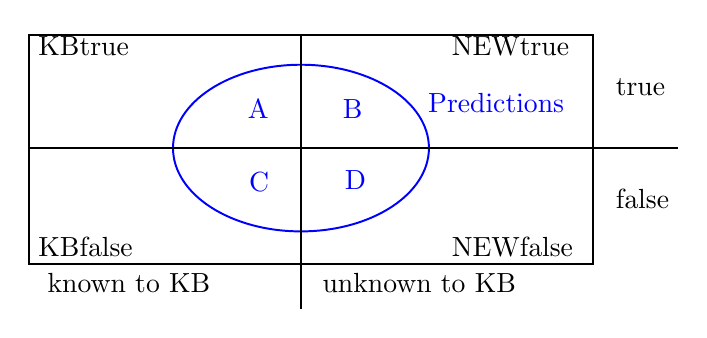
\begin{tikzpicture}

% Fabian: Keep figure in two colors.
% Even if printed in black and white, it's still clear enough

  \path[draw=blue, line width=0.7086614168764338] (3.708333, -1.458333) ellipse (1.625000 and 1.058333);
  \node[above, right, color=blue, font=] at (5.2000, -0.88333) {Predictions};
  \node[above, right, color=blue, font=] at (2.908333, -0.958333) {A};
  \node[above, right, color=blue, font=] at (4.116667, -0.966667) {B};
  \node[above, right, color=blue, font=] at (2.925000, -1.891667) {C};
  \node[above, right, color=blue, font=] at (4.141667, -1.866667) {D};
  \node[above, right, color=black, font=] at (0.250000, -0.166667) {KBtrue};
  \node[above, right, color=black, font=] at (0.250000, -2.708333) {KBfalse};
  \node[above, right, color=black, font=] at (5.500000, -0.166667) {NEWtrue};
  \node[above, right, color=black, font=] at (5.500000, -2.708333) {NEWfalse};
  \node[above, right, color=black, font=] at (7.583333, -0.683333) {true};
  \node[above, right, color=black, font=] at (7.583333, -2.100000) {false};
  \node[above, right, color=black, font=] at (0.366667, -3.166667) {known to KB};
  \node[above, right, color=black, font=] at (3.858333, -3.166667) {unknown to KB};
  \path[draw=black, line width=0.7086614168764338] (0.250000, -0.016667) rectangle (7.416667, -2.933333);
  \draw[draw=black, line width=0.7086614168764338] (0.250000, -1.458333) -- (8.500000, -1.458333);
  \draw[draw=black, line width=0.7086614168764338] (3.708333, -0.025000) -- (3.708333, -3.500000);
\end{tikzpicture}
}

}

\www{
\paragraph{Goal} 
Our goal is to find rules that make true predictions that go beyond the current KB. 
In the figure, we wish to maximize the area B, and to minimize the area D. 
There are two obvious challenges in this context: First, the areas NEWtrue and NEWfalse are unknown. 
So if we wish to maximize B at the expense of D, we are operating in an area outside our KB. 
We would want to use the areas KBtrue and KBfalse to estimate the unknown area. 
This, however, leads to the second challenge: Semantic KBs do not contain negative evidence. 
Thus, the area KBfalse is empty. In the following, we discuss different measures that address these challenges.
}

% \www{
% \paragraph{Support} 
% The \emph{support} of a rule quantifies the number of correct predictions, i.e., the size of A. There are several ways to define the support: It can be the number of instantiations of the rule that appear in the KB. This is what our analogy to association rule mining \cite{AgrImiSwa93} suggests (Section \ref{sec:preliminaries}). This measure, however, is not monotonic if we add atoms to the body. Consider, for example, the rule
% \indented{
%   \emph{marriedTo(}$x,y) \Rightarrow$ \emph{marriedTo(}$y,x$)
% }
% If we add \emph{hasGender($x$,male)} to the body, the number of instantiations that are in the KB decreases. If we add an atom with a fresh variable, e.g., \emph{hasFriend($x$,$z$)}, to the body, the number of instantiations increases for every friend of $x$. This is true even if we add another atom with $z$ to make the rule closed.\
% Alternatively, we can count the number of facts in one particular body atom.
% This definition, however, depends on the choice of the body atom, so that the same rule can have different supports. We can also count the number of facts of the head atom.
% This measure decreases monotonically if more body atoms are added 
% and avoids equivalent rules with different support values. With this in mind, we define the support of a rule as the number of distinct pairs of subjects and objects in the head of all instantiations that appear in the KB:
% \[supp(\vec{B} \Rightarrow r(x,y)) := \#(x,y): \exists z_1,...,z_m: \vec{B} \wedge r(x,y)\]
% where $z_1,...,z_m$ are the variables of the rule apart from $x$ and $y$.
% }

\www{
\paragraph{Support} 
The \emph{support} of a rule quantifies the number of correct predictions, i.e., the size of A. 
There are several ways to define the support: It can be the number of instantiations of the rule that appear in the KB. 
%This is what our analogy to association rule mining \cite{AgrImiSwa93} suggests (Section \ref{sec:preliminaries}). \comment{Katja}{Remove this sentence if the section about association rule mining is removed permanently.}
This measure, however, is not monotonic if we add atoms to the body. Consider, for example, the rule
\indented{
  \emph{marriedTo(}$x,y) \Rightarrow$ \emph{marriedTo(}$y,x$)
}
If we add \emph{hasGender($x$,male)} to the body, the number of instantiations that are in the KB decreases. 
If we add an atom with a fresh variable, e.g., \emph{hasFriend($x$,$z$)}, to the body, the number of instantiations increases for every friend of $x$. 
This is true even if we add another atom with $z$ to obtain a closed rule.\
Alternatively, we can count the number of facts in one particular body atom.
This definition, however, depends on the choice of the body atom, so that the same rule can have different supports. 
We can also count the number of facts of the head atom.
This measure decreases monotonically if more body atoms are added and avoids equivalent rules with different support values. 
With this in mind, we define the support of a rule as the number of distinct pairs of subjects and objects in the head of all instantiations that appear in the KB:
\[supp(\vec{B} \Rightarrow r(x,y)) := \#(x,y): \exists z_1,...,z_m: \vec{B} \wedge r(x,y)\]
where $z_1,...,z_m$ are the variables of the rule apart from $x$ and $y$. }
Note that the support is defined even for rules that are not closed.


% \www{
% \paragraph{Head Coverage} %\comment{check again}
% % Support is an absolute number. This means that a user who thresholds on support has to know the absolute size of the KB to give meaningful values. 
% % To avoid this, we also need to define a proportional version of support, the \emph{head coverage}. It is the proportion of pairs from the head relation that are covered by the predictions of the rule:
% % \[hc(\vec{B} \Rightarrow r(x,y)) := \frac{supp(\vec{B} \Rightarrow r(x,y))}{\#(x,y) : r(x,y)}\]
% Support is an absolute number. This means that a user who thresholds on support has to know the absolute size of the KB to give meaningful values. 
% To avoid this, we also define a proportional version of support. A naive way would be to use the absolute number of support, as defined in the previous paragraph, over the size of the KB. 
% In this case, however, relations that do not have many facts (either because of the incompleteness of the KB or because of their nature), will not be considered in the head of rules,
% i.e. we will not learn rules predicting such relations. Therefore, we propose to use the notion of \emph{head coverage}. 
% This is the proportion of pairs from the head relation that are covered by the predictions of the rule
% % Head coverage is the proportion of pairs from the head relation that are covered by the predictions of the rule:
% \[hc(\vec{B} \Rightarrow r(x,y)) := \frac{supp(\vec{B} \Rightarrow r(x,y))}{\#(x',y') : r(x',y')}\]
% }


\www{
\paragraph{Head Coverage}
Support is an absolute number. This means that a user defining thresholds on support has to know the absolute size of the KB to give meaningful values. 
To avoid this, we propose a proportional version of support. A naive way would be to use the absolute number of support, as defined in the previous paragraph, over the size of the KB. 
In this case, however, relations that do not have many facts (either because of the incompleteness of the KB or because of their nature) will not be considered in the head of the rules,
i.e., we will not learn rules predicting such relations. Therefore, we propose to use the notion of \emph{head coverage}:
\[hc(\vec{B} \Rightarrow r(x,y)) := \frac{supp(\vec{B} \Rightarrow r(x,y))}{size(r)}\]
}

with $size(r) := \#(x',y') : r(x',y')$ denoting the number of facts in relation $r$.

Head coverage quantifies the percentage of the known true facts that are implied %(for the case of closed rules) %or can possibly be implied (for the case of not yet closed rules)
% Fabian: I think that this description is sufficient. The mroe precise one risks confusing readers.
by the rule.
Head coverage can be a measure of statistical significance for any measure used to evaluate the quality of a rule. 
\comment{Fabian}{I am not sure about this. Could you explain? If it is not crucial here, I would omit it at this position.}



\www{
\paragraph{Negative Examples} 
The central challenge of our setting is to provide counter-examples for the rule mining. 
These can take the role of KBfalse, so that we can estimate the areas NEWtrue and NEWfalse. 
There are several approaches to this problem: The standard confidence, the standard positive-only learning evaluation score of ILP, and the partial completeness assumption that we propose. 
}
We will now present these approaches in detail.

% \www{
% \paragraph{Standard Confidence} 
% The standard confidence measure takes all facts that are not in the KB (i.e., NEWtrue and NEWfalse) as negative evidence. 
% Thus, the standard confidence of a rule is the ratio of its predictions that are in the KB, i.e., the share of A in the set of predictions:
% \[conf(\vec{B} \Rightarrow r(x,y)) := \frac{supp(\vec{B} \Rightarrow r(x,y))}{\#(x,y): \exists z_1,...,z_m: \vec{B}}\]
% %\[conf(\vec{B} \Rightarrow r(x,y)) := \frac{supp(\vec{B} \Rightarrow r(x,y))}{supp(\vec{B})}\]
% The standard confidence is blind to the distinction between ``false'' and ``unknown''. Thus, it implements a closed world setting. It mainly describes the known data and penalizes rules that make a large number of predictions in the unknown region. We, in contrast, aim to maximize the number of true predictions that go beyond the current knowledge. We do not want to describe data, but to predict data.
% }



\www{
\paragraph{Standard Confidence} 
The standard confidence measure takes all facts that are not in the KB (i.e., NEWtrue and NEWfalse) as negative evidence. 
Thus, the standard confidence of a rule is the ratio of its predictions that are in the KB, i.e., the share of A (KBtrue) in the set of predictions:
%\[conf(\vec{B} \Rightarrow r(x,y)) := \frac{supp(\vec{B} \Rightarrow r(x,y))}{\#(x,y): \exists z_1,...,z_m: \vec{B}}\]
}

%\comment{Katja}{I prefer the second one.}
\[conf(\vec{B} \Rightarrow r(x,y)) := \frac{\#(x,y): \exists z_1,...,z_m: \vec{B} \wedge r(x,y)}{\#(x,y): \exists z_1,...,z_m: \vec{B}}\]
%\[conf(\vec{B} \Rightarrow r(x,y)) := \frac{supp(\vec{B} \Rightarrow r(x,y))}{supp(\vec{B})}\]

Standard confidence is the measure traditionally used in association rule mining and market basket analysis, where a Closed World Assumption (CWA) is made: 
if there is no evidence in any of the transactions of the database that a user bought a specific product, then this user did not buy the product.
Although natural for the market basket analysis scenario, standard confidence fails to distinguish between ``false'' and ``unknown'' facts, 
which makes it inappropriate for a scenario with Open World semantics, like ours. Moreover, we also persue a different goal than market basket analysis:
we aim to maximize the number of true predictions that go beyond the current knowledge, whereas market basket analysis usually tries to mine rules that can describe data that is already known. 






\www{
\paragraph{Positive-Only Learning} 
For cases where the KB does not contain negative examples, Muggleton has developed a \emph{positive-only learning evaluation score} for ILP \cite{Muggleton:1996:LPD:647996.742465},\cite{usir1753}. 
It takes random facts as negative evidence:
\[
 Score = log(P)-log\frac{R+1}{Rsize+2}-\frac{L}{P}
\]
Here, $P$ is the number of known true facts covered (KBtree, or A resp., in Figure~\ref{fig:prediction}), $R$ is the number of randoms covered, $Rsize$ is the total number of randoms and $L$ is the number of atoms in the hypotheses. 
The intuition is that a good rule should cover many positive examples, and few or no randomly generated examples. This ensures  
that the rule is not overly general. Furthermore, the rule should use as few atoms as possible, and thus achieve a high compression. This measure is implemented (among others) in the ALEPH system.
}


% \www{
% \paragraph{Partial Completeness} 
% We propose to generate negative evidence by the \emph{partial completeness assumption} (PCA).
% This is the assumption that if $r(x,y) \in$ \emph{KBtrue} for some $x,y$, then
% \[\forall y': r(x,y') \in \mbox{\emph{KBtrue}} \cup \mbox{\emph{NEWtrue}} \Rightarrow r(x,y') \in \mbox{\emph{KBtrue}}\] 
% In other words, we assume that if the database knows some $r$-attribute of $x$, then it knows all $r$-attributes of $x$. This assumption is certainly true for functional relations $r$, 
% such as birth dates, capitals, etc. Thanks to the FUN-Property (see Section \ref{sec:model}), it is also true for inverse-functional relations, such as \emph{owns}, \emph{created}, etc. 
% The assumption is also true in the vast majority of cases for relations that are not functional, but that have a high functionality. 
% Even for other relations, the PCA is still reasonable for knowledge bases that have been extracted from a single source (such as DBpedia and YAGO). 
% These usually contain either all $r$-values or none for a given entity.
% }


\paragraph{Partial Completeness} 
We propose to generate negative evidence by means of the \emph{partial completeness assumption} (PCA).
This is the assumption that if $r(x,y) \in$ \emph{KBtrue} for some $x,y$,
%and $x$ is the input variable, 
% Fabian: we already said that all relations are more functional than inverse functional
then
\[\forall y': r(x,y') \in \mbox{\emph{KBtrue}} \cup \mbox{\emph{NEWtrue}} \Rightarrow r(x,y') \in \mbox{\emph{KBtrue}}\] 
%In other words, we assume that if the database knows some $r$-attribute of $x$, then it knows all $r$-attributes of $x$. 
%In other words, we assume that if the database knows some entity for the output variable $y$ for a given relation $r$ and entity of the input variable $x$, 
%then it knows all possible entities for the  output variable $y$ for these $r$ and $x$.
%\comment{Katja}{The term ``$r$-attribute of $x$'' is not intuitive for the reader as it has not been formally introduced, and the term attribute occurs only here. I suggest to replace it.}
% Fabian: I gave it another try, without the input and output:
In other words, we assume that if we know one $y$ for a given $x$, then we know all $y$ for that $x$.

This assumption is certainly true for functional relations $r$, such as \emph{birthdates} and \emph{capitals}.
Thanks to the FUN-property, the assumption is also true for inverse-functional relations, such as \emph{owns} and \emph{created}.
%, with the difference that in this case $x$ is the output variable and $y$ the input variable.
%, with the difference that in this case we assume that we know all $r$-attributes of $y$ (since $y$ is the input variable in this case).
The assumption is also true in the vast majority of cases for relations that are not functional, but that have a high functionality. 
Even for other relations, the PCA is still reasonable for knowledge bases that have been extracted from a single source (such as DBpedia and YAGO), as we shall see. 
%These usually contain either all $r$-values or none for a given entity. \comment{Katja}{Likewise, the term ``$r$-values'' is not introduced.}
We present an experimental evaluation of the PCA in Section~\ref{sec:experimentsPCA}.

% \www{
% \paragraph{PCA Confidence} 
% Under the PCA, we normalize the confidence not by the entire set of facts, but by the set of facts of which we know that they are true, together with the facts of which we assume that they are false. If the head atom of the rule is $r(x,y)$, then this set is just the set of facts $\{ r(x,y') : r(x,y') \in \mathcal{K}\}$. Thanks to the FUN-Property, the PCA is always applied to the first argument of the head atom:
% %\[pcaconf(\vec{B} \Rightarrow r(x,y)) := \frac{\#(x,y): \exists z_1,...,z_m: \vec{B} \wedge r(x,y)}{\#(x,y): \exists z_1,...,z_m,y': \vec{B} \wedge r(x,y')}\]
% \[pcaconf(\vec{B} \Rightarrow r(x,y)) := \frac{supp(\vec{B} \Rightarrow r(x,y))}{\#(x,y): \exists z_1,...,z_m,y': \vec{B} \wedge r(x,y')}\]
% We show in our experiments that the PCA confidence identifies much more productive rules than the other measures.
% }



\paragraph{PCA Confidence} 
\label{pcaConf}
Under the PCA, the denominator of the confidence will not be the size of the entire set of facts that the body of the rule produces, 
but the number of facts that we know to be true together with the facts that we assume to be false. 
\comment{Fabian}{Important fix here: Christina found that the denominator should count $\#(x,y)$, and not $\#(x,y')$.}

% If the head atom of the rule is $r(x,y)$, then this set is just the set of facts $\{ r(x,y') : r(x,y') \in \mathcal{K}\}$. 
% The PCA confidence for a rule with $x$ as the input variable is defined as:
% \[
% \small \hspace*{-1ex}
% conf_{PCA}(\vec{B} \Rightarrow r(x,y)) := \frac{supp(\vec{B} \Rightarrow r(x,y))}{\#(x,y): \exists z_1,...,z_m,y': \vec{B} \wedge r(x,y')}
% \]
% \comment{Katja}{If we replace the formula for the standard confidence, we should use the same notation here:
\[
\small \hspace*{-2ex}
conf_{PCA}(\vec{B} \Rightarrow r(x,y)) := \frac{\#(x,y): \exists z_1,...,z_m: \vec{B} \wedge r(x,y)}{\#(x,y): \exists z_1,...,z_m,y': \vec{B} \wedge r(x,y')}
\]
%}
This confidence normalizes the support by the number of pairs $(x,y)$ for which there exists a $y'$ with $r(x,y')$, i.e., for which we assume that the KB knows all such $y'$.
\comment{Chris}{Think about if you want to include the following one.} 
\comment{Katja}{I suggest to remove it because we will have a detailed discussion in the experiments and do not need it already here.}
The PCA confidence can be seen as a process in which we first take a biased sample of the body (those facts containing entities for the $x$ variable that appear also in the head)
and then calculate the standard confidence over this sample. 
The fact that our sample is biased implies that PCA confidence might not be a good estimator of the actual predictive power of the rule (precision).
However, our experiments show that overall PCA confidence identifies much more productive rules than the other measures and it also correlates with precision better than the standard confidence.


%- - - - - - - - - - - - - - - - - - - - - - - - - - - - - - 
\section{AMIE}
\label{sec:alg}
% !TEX root = main.tex

\www{
%After having outlined the preliminaries and the mining model in Sections~\ref{sec:preliminaries} and \ref{sec:pca},
We now outline the core algorithm of AMIE and its implementation.
%Again, we follow the explications in \cite{amie}.
We follow the explications in \cite{amie} and extend them with further explanations and details.
}

\www{
%- - - - - - - - - - - - - - - - - - - - - - - - - - - - - -
\subsection{Algorithm}
\label{subsec:algorithm}
\comment{R2}{Similarly, the Algorithm 2 is not very accurate. It would be clearer if "distinct" is added on line 15: "for all distinct x $\in$ SELECT ?x FROM K WHERE q do." (In contrast, the DISTINCT in the query on the top of Page 11 is redundant).}

\comment{R3}{Here are some of my criticisms, which apply to Section 5 on AMIE - your previous work:
1.Algorithm 1 is too high level and as such it leaves too much unexpressed (e.g. "execute in parallel", "is not pruned for output").
2.      SQL and SPARQL are presented at page 11 only to say that they are discarded for a custom implementation.
3.      The "vanilla in-memory database" implementation is too informally described (e.g.: each "index is a map from the first item to a map from the second item to a set of the third item": a more formal description and a figure, please!
}

\paragraph{Goal} Our goal is to mine rules of the form defined in Section~\ref{sec:preliminaries}.
One of the main problems of any mining approach is to find an efficient way to explore the search space. The naive algorithm of enumerating all possible rules is infeasible for large KBs.
Hence, we explore the search space by iteratively extending rules by \emph{mining operators}.
}

\www{
\paragraph{Mining Operators}
We see a rule as a sequence of atoms. The first atom is the head atom and the others are the body atoms. In the process of traversing the search space, we can extend a rule by using one of the following operators:
\begin{enumerate}
\item \textbf{Add Dangling Atom ($\mathcal{O}_D$})\\
This operator adds a new atom to a rule. The new atom uses a fresh variable for one of its two arguments. The other argument is a variable
that is shared with the rule, i.e., it occurs in some other atom of the rule.
\item \textbf{Add Instantiated Atom ($\mathcal{O}_I$})\\
This operator adds a new atom to a rule that uses an entity for one argument and shares the other argument (variable or entity) with the rule.
\item \textbf{Add Closing Atom ($\mathcal{O}_C$})\\
This operator adds a new atom to a rule so that both of its arguments are shared with the rule.
\end{enumerate}
By repeated application of these operators, we can generate the entire space of rules as defined in Section~\ref{sec:preliminaries}.
The operators generate even more rules than those that we are interested in, because they also produce rules that are not closed.
An alternative set of operators could consist of $\mathcal{O}_D$ and an operator for instantiation.
But these operators would not be monotonic, in the sense that an atom generated by one operator can be modified in the next step by the other operator.
Therefore, we chose the above 3 operators as a canonic set.
}


\paragraph{Algorithm} \label{algo}
Algorithm~\ref{rm} sketches our approach to mine rules. The algorithm maintains a queue of rules, 
which initially contains all possible head atoms, that is,
all rules of size 1.
The algorithm iteratively dequeues a rule from the queue. If the rule 
meets certain criteria (Lines 6 and 7), then it is output.
% \comment{Chris}{its quality is evaluated in terms of (PCA) confidence and if it passes the corresponding threshold} \comment{Luis: }{We threshold on PCA confidence
%  only for AMIE+}\comment{Chris}{so, are we going to output a rule with confidence 0\%?},
Then, the algorithm applies all mining operators to the rule. This results in more rules which are added to 
the queue if they pass the head coverage threshold $\theta$ (Lines 9 to 15).
This process is repeated until the queue is empty. 
To speed up the process, our implementation parallelizes Algorithm~\ref{rm}, that is, the main loop (Lines 4 to 16) runs
in multiple threads. 
This achieved by synchronizing the access to the centralized queue from which the threads dequeue and enqueue.
We do not feed predictions of the rules back into the KB. All measures (such as confidence and support) are always computed on the original KB.


% \comment{Chris}{about the figure: shouldn't there be a line stating that the rule is evaluated somehow?}
% Fabian: We discussed this and agreed to leave it as it is until the need arises.

\begin{algorithm}
\caption{Rule Mining}
\label{rm}
\begin{algorithmic}[1]
\Function{AMIE}{KB $\mathcal{K}$, $\theta$, $minConf$}
    \State $q = \langle [r_1(x,y), r_2(x,y) \dots r_m(x,y)] \rangle$
    \State $out = \langle \rangle$
	\While{$\neg q$\emph{.isEmpty}()}
	  \State $r = q.$\emph{dequeue}()
	  \If{$AcceptedForOutput(r, out, minConf)$}
	    \If{$r \notin out$}
	      \State $out.$\emph{add}$(r)$
	    \EndIf
	  \EndIf
	  \ForAll{operators $o$}
	    \ForAll{rules $r' \in o(r)$}
		  \If{$hc(r') \ge \theta$}
		    \If{$r' \notin q$}
		      \State $q.$\emph{enqueue}$(r')$
		    \EndIf
		  \EndIf
		\EndFor
	  \EndFor
	\EndWhile
    \State \Return $out$
\EndFunction
\end{algorithmic}
\end{algorithm}

\begin{algorithm}
\caption{Routine to decide to output a rule}
\label{pfo}
\begin{algorithmic}[1]
\Function{AcceptedForOutput}{rule $r$, $out$, $minConf$}
    \If{$r$ is not closed $\vee\; pcaconf(r) < minConf$}
      \State \Return $false$
    \EndIf 
    \State $parents = parentsOfRule(r, out)$
    \ForAll{$r_p \in parents$}
      \If{$pcaConf(r) < pcaconf(r_p)$}
	\State \Return $false$
      \EndIf
    \EndFor
    \State \Return $true$
\EndFunction
\end{algorithmic}
\end{algorithm}

% \www{
% \paragraph{Pruning} If executed naively, our algorithm will have prohibitively high runtimes. The instantiation operator $\mathcal{O}_I$, in particular, generates atoms in the order of $|\mathcal{R}| \times |\mathcal{E}|$. We first observe that we are usually not interested in rules that cover only very few facts of the head relation.
% % \comment{Katja}{Would a proper definition of what ''instances`` means in this context be useful?}
% % Fabian: switched to "facts of head relation"
% Rules that cover, for example, less than 1\% of the facts of the head relation can safely assumed to be marginal. Therefore, we set $\theta=0.01$ as a lower bound for the head coverage. We observe that head coverage decreases monotonically as we add more atoms. This allows us to safely discard any rule that trespasses the threshold (Lines 11 and 12).
% % \comment{Katja}{Maybe add the threshold itself to the pseudocode algorithm.}
% % Fabian: Yes, this is an option. I wanted to keep the algorithm general, and outsource the definition of "pruning" to this paragraph here. This is because the algorithm is first discussed in generality in the previous section.
% }


%\comment{Katja}{How about some restructuring (introducing subsections) that shows more clearly what paragraph belongs where, i.e., at the moment ''Algorithm``, ''Pruning``, ''Reducing the output size``, etc. are all on the same level (all paragraphs).}

\subsection{Stages of Rule Mining}

\subsubsection{Output a Rule}  
\label{subsubsec:whenToOutput}
Algorithm~\ref{pfo} describes the routine to decide if a rule should be output or 
not once it has been dequeued. If the rule is not closed (See Section~\ref{subsec:rules}) or 
its PCA confidence is below the given confidence threshold, the algorithm discards it for output. 
Recall that AMIE is conceived to mine rules that can predict concrete facts and therefore, thus non-closed rules are
seen as intermediate steps. Moreover, the PCA confidence is only defined for closed rules.
It is important to remark, that the confidence threshold is enforced 
very late in the rule mining process, i.e., right before reporting the rule. 
This occurs because confidence is not monotonic, that is, the addition of atoms to a rule
can both increase or decrease its confidence. This means that confidence is not suitable for accurate
pruning. Enforcing the confidence threshold at the end also implies that
the runtime of AMIE is not affected by the magnitude of this value. For this reason, 
the confidence threshold is an optional argument for AMIE. If omitted, the system assumes a value of 0. 

If the rule is closed and confident enough, Algorithm~\ref{pfo} then applies a \emph{skyline technique} (Lines 5 to 10)
to reduce the output. If a rule $B_1 \wedge ... \wedge B_n \wedge B_{n+1} \Rightarrow H$ does not have larger confidence
than its parent rule $B_1 \wedge ... \wedge B_n \Rightarrow H$, then we do not output the longer rule.
Since support and head coverage are monotonic metrics, we know that the child rule will never have a higher value than its parent rule. 
If the child rule has lower confidence, then its quality is worse in all aspects and there is 
no reason to include it in the output.
In addition, notice that a rule can have multiple parents, for instance, the rule $actedIn(x,y) \wedge directedIn(x,y) \Rightarrow created(x,y)$
can be derived by applying a closing-atom operator $\mathcal{O}_C$ to either $actedIn(x,y) \Rightarrow created(x,y)$ or
$directedIn(x,y) \Rightarrow created(x,y)$. While in practice the longer rule is derived from one of those rules, AMIE
finds all its potential parents (Line 5) and applies the skyline technique for each of them (Lines 6 to 10), i.e., the child
rule must have higher confidence than all its parents to be accepted.
We emphasize that the skyline technique is only applied to prune the output. 
Since confidence can increase with the addition of atoms, we should still use the longer rule 
for further refinement.

% We never enqueue a rule that is already in the queue. It is expensive to check two rules for equality.
% However, it is easy to compute the support for each rule. Two rules can only be equal if they have the same head relation and
% the same support. This reduces the set of rules that have to be checked. If a rule is duplicate, we do not enqueue it (lines 11 and 12 in Algorithm~\ref{rm}).
% 
% Since our algorithm performs a breadth-first-search, we can be sure that for any new rule, its potential duplicates will still be in the queue.
% When we dequeue a rule with $n$ atoms, no rule with $n+1$ atoms has ever been dequeued. Thus, when we apply the mining operators to the rule with $n$ atoms, and generate a rule with $n+1$ atoms,
% any potential duplicate of that new rule must be in the queue.


\subsubsection{Pruning} 
\label{subsubsec:pruning}
\www{
If executed naively, Algorithm~\ref{rm} will have prohibitively high runtimes.
The instantiation operator $\mathcal{O}_I$, in particular, generates atoms in the order of $|\mathcal{R}| \times |\mathcal{E}|$.
We first observe that we are usually not interested in rules that cover only very few facts of the head relation.
Rules that cover, for example, less than 1\% of the facts of the head relation can safely be assumed to be marginal.
Therefore, we choose $\theta=0.01$ as a lower bound for the head coverage. We observe that head coverage decreases monotonically as we add more atoms.
This allows for safely discarding any rule that trespasses the threshold (lines 11 and 12 in Algorithm~\ref{rm}).
}
Recall from Section~\ref{subsec:statSignificance} that support and head coverage are defined even for rules that are not yet closed, allowing for early pruning.

\subsubsection{Duplicate elimination} 
\label{subsubsec:duplicateElimination}
As mentioned in Section~\ref{subsubsec:whenToOutput} a rule can be derived in multiple ways.
For example, the rule $actedIn(x,y) \wedge directedIn(x,y) \Rightarrow created(x,y)$ can result from the application
of the operator $\mathcal{O}_C$ to both $actedIn(x,y) \Rightarrow created(x,y)$ and $directedIn(x,y) \Rightarrow created(x,y)$.


We never enqueue a rule that is already in the queue. It is expensive to check two rules for equality.
However, it is easy to compute the support for each rule. Two rules can only be equal if they have the same head relation and
the same support. This reduces the set of rules that have to be checked. If a rule is duplicate, we do not enqueue it (lines 11 and 12 in Algorithm~\ref{rm}).

Since our algorithm performs a breadth-first-search, we can be sure that for any new rule, its potential duplicates will still be in the queue.
When we dequeue a rule with $n$ atoms, no rule with $n+1$ atoms has ever been dequeued. Thus, when we apply the mining operators to the rule with $n$ atoms, and generate a rule with $n+1$ atoms,
any potential duplicate of that new rule must be in the queue.

% \paragraph{Reducing the Output Size}  We can reduce the number of output rules in many different ways.
% If a rule $B_1 \wedge ... \wedge B_n \wedge B_{n+1} \Rightarrow H$ does not have larger confidence
% than the rule $B_1 \wedge ... \wedge B_n \Rightarrow H$, then we do not output the longer rule (lines 6 and 7 in Algorithm~\ref{rm}).
% Since head coverage is monotonic, we know that the longer rule will have smaller head coverage than its parent rule, and we also do not expect it to be of higher quality because its confidence is lower. %behave better quality-wise.
% Therefore, there is no reason to include the longer rule in the output.
% However, since confidence is not monotonic, we can possibly obtain rules of higher confidence by adding even more atoms.
% Therefore, we still use the longer rule for further refinement.
% 
% We never enqueue a rule that is already in the queue. It is expensive to check two rules for equality.
% However, it is easy to compute the support for each rule. Two rules can only be equal if they have the same head relation and
% the same support. This reduces the set of rules that have to be checked. If a rule is duplicate, we do not enqueue it (lines 11 and 12 in Algorithm~\ref{rm}).
% 
% Since our algorithm performs a breadth-first-search, we can be sure that for any new rule, its potential duplicates will still be in the queue.
% When we dequeue a rule with $n$ atoms, no rule with $n+1$ atoms has ever been dequeued. Thus, when we apply the mining operators to the rule with $n$ atoms, and generate a rule with $n+1$ atoms,
% any potential duplicate of that new rule must be in the queue.




% \www{
% The monotonicity of head coverage gives us another opportunity to prune: If a rule $B_1 \wedge ... \wedge B_n \wedge B_{n+1} \Rightarrow H$ does not have larger confidence
% than the rule $B_1 \wedge ... \wedge B_n \Rightarrow H$, then we do not output the longer rule.
% This is because both the confidence and the head coverage of the longer rule are necessarily dominated by the shorter rule.
% This way, we can reduce the number of produced rules (Lines 6 and 7).
% }
%
% \www{
% Last, we never enqueue a rule that is already in the queue. It is expensive to check two rules for equality.
% However, it is easy to compute measures such as head coverage, confidence, and PCA confidence for each rule. Two rules can only be equal if they have the same values for these measures.
% This restricts the rules that have to be checked. If a rule is duplicate, we do not enqueue it (Lines 11 and 12).
% We can be sure that any potential duplicates will still be in the queue. This is because the length of the rules increases monotonically: When we dequeue a rule with $n$ atoms, no rule with $n+1$ atoms has ever been dequeued. Thus, when we apply the operators to the rule with $n$ atoms, and generate a rule with $n+1$ atoms, any potential duplicate of that new rule must be in the queue.
% }

\ignore{
% Fabian: Problem solved. Thanks, Luis!
\comment{Fabian}{Problem: what if the duplicate rule has already been dequeued by some other thread?}
\comment{Katja}{Use a pointer over the queue that points to the next item to be dequeued by the next thread. The first positions correspond to rules that are currently considered by active threads. Remove the rule when the thread is finished. Check all rules for duplicates when trying to add a new rule to the queue.}
\comment{Luis}{We use a set that guarantees insertion order at iteration time (LinkedHashSet) to explore the space in a breath search fashion. That means that by the time the first of size n is dequeued, all rules of size n are already in the
queue and duplicates have been already pruned.}
}

% \www{
% \paragraph{Projection Queries}
% No matter what operator is applied in particular, the algorithm needs to choose a relation for the new atom that is added to the rule. In addition,
% the instantiation operator $\mathcal{O_I}$ also allows the choice of an entity. In order to select only relations and entities that will fulfill the head coverage constraint, we rely on the KB to answer \emph{projection queries}. These are queries of the form
% \indented{SELECT $?x$ WHERE $H \wedge B_1 \wedge ... \wedge B_n$\\
% HAVING COUNT($H$)$\geq k$}
% where $B_1, ..., B_n$ are atoms and $k$ is a natural number. $H$ is the \emph{projection atom} on which we project. $?x$ is the \emph{selection variable}. It is a variable that appears in one or more atoms at the position of one of the arguments or at the position of the relation (as it is common in SPARQL\footnote{\url{http://www.w3.org/TR/rdf-sparql-query/}}). Such queries select an entity or relation $x$ such that the result of the query $H \wedge B_1 \wedge ... \wedge B_n$ on the KB contains more than $k$ distinct query answers for $H$.
% }

%\comment{Katja}{Some hierarchy of paragraphs/subsections would probably also be useful in the following.}
\subsection{Count-Projection Queries}
\label{projectionQueries}

%\paragraph{Projection Queries}
No matter what operator is applied in particular, the algorithm needs to choose a relation for the new atom that will be added to the rule.
In addition, the instantiation operator $\mathcal{O_I}$ also allows the choice of an entity.
In order to select only relations and entities that will fulfill the head coverage constraint, we rely on the KB to answer \emph{count-projection queries}.
These are queries of the form
\indented{SELECT $?x$, COUNT($H$) \\
WHERE $H \wedge B_1 \wedge ... \wedge B_n$\\
SUCH THAT COUNT($H$)$\geq k$}
%\comment{Katja}{It still looks weird to have a HAVING clause without a GROUP BY.}
where $B_1, ..., B_n$ are atoms and $k$ is a natural number.
% \comment{Katja}{Strictly speaking we project on $?x$ as this is the only value in the select clause. It would be safe to say that we project on $?x$ but select (have an additional condition) on $H$. So, $H$ could be the ``group atom''.}
% \comment{Luis :}{I agree with Katja. We should be strict in notation. I wonder whether we should stop calling them ``projection queries''
% as it sounds too generic.}
$?x$ is the \emph{selection variable}.
It is a variable that appears in one or more atoms at the position of one of the arguments or at the position of the relation (as it is common in SPARQL~\cite{sparql}). 
Such queries select an entity or relation $x$ such that the result of the query $H \wedge B_1 \wedge ... \wedge B_n$ on the KB contains more than $k$ distinct query answers
for the \emph{group atom} $H$. The group atom corresponds to the head of the rule.
% Fabian: we never said it, so the reader cannot recall
%Recall that the expression COUNT($H$) binds to the support
%of the whole query pattern for each value of the selection variable $?x$.

We will discuss the implementation of such queries and their relation to SPARQL and SQL queries below. For now, we will use the above pseudo-syntax.

\paragraph{Using Projection Queries} Projection queries allow us to select the relationship for the operators $\mathcal{O_D}$, $\mathcal{O_I}$, and $\mathcal{O_C}$ in such a way
that the head coverage of the resulting rule is above $\theta$.
 This works by firing a projection query of the form
\\ \\
SELECT $?r$, COUNT($H$)\\
WHERE $H \wedge B_1 \wedge ... \wedge B_{n-1}\; \wedge\; ?r(X,Y)$\\
SUCH THAT COUNT($H$)$\geq k$
\\ \\
%\comment{Katja}{HAVING without GROUP BY, see above}
where $k := \theta \times size(H)$. $X$ and $Y$ are variables or constants, depending on the type of atoms that the operator generates.
The results for $?r$ are the relations that, once bound in the query, ensure that the head coverage of the rule $B_1 \; \wedge ... \wedge B_{n-1} \;\wedge\; ?r(X,Y) \Rightarrow H$ is greater than $\theta$.
For instance, assume
Algorithm~\ref{rm} dequeues the following intermediate non-closed rule for further refinement.

\begin{center}
\emph{isMarriedTo}$(x,z) \Rightarrow $ \emph{livesIn}$(x,y)$
\end{center}

\noindent
The application of the operator $\mathcal{O_D}$ will fire queries of the form:\\ \\
SELECT $?r$, COUNT($livesIn(x,y)$)\\
WHERE $livesIn(x,y) \; \wedge \; isMarriedTo(x,z) \wedge ?r(X, Y)$\\
SUCH THAT COUNT($livesIn(x,y)$)$>= k$\\

\noindent with $?r(X, Y) \in \{?r(x,w), ?r(z,w), ?r(w,x), ?r(w,z) \}$, i.e., each possible join combination of a new dangling atom,
where $w$ is an arbitrary fresh variable. For intermediate rules, dangling atoms are joined on the non-closed variables; $z$ and $y$ in this example.
% \comment{Fabian}{$w$ does not appear at all! This has to be rewritten!} \comment{Katja}{Has this been rewritten and the comment remained?}
If the rule is closed, dangling atoms are joined on all the variables appearing in the rule.
%then the system will fire queries for every possible join combination of the new dangling atom with any (all) of the variables appearing in the rule.
%\comment{Katja}{Wouldn't it be nice to have an example here for what ``for every possible join combination'' means in practice, e.g., in relation to the above example with $livesIn$?}
%If the rule is closed, then the new atom is joined with all the variables in the rule.
%\comment{Katja}{How can the rule be closed if the queue in Algorithm 1 contains only non-closed rules? Shouldn't $\mathcal{O_D}$ leave a non-closed variable?}
%\comment{Chris}{In the queue we can have both closed and non closed rules that we want to refine further.}

In the same fashion, when applying the $\mathcal{O_C}$ to our example, the atom $?r(X, Y)$ can take values in $\{ ?r(z,y), ?r(y,z) \}$.
% \\ \\
% SELECT $?r$, COUNT($livesIn(x,y)$)\\
% WHERE $livesIn(x,y) \wedge isMarriedTo(x,z) \wedge\; ?r(z,y)$\\
% SUCH THAT COUNT($livesIn(x,y)$)$>= k$
% \\ \\
%\comment{Katja}{HAVING without GROUP BY, see above}
%is one of the ways to apply the operator $\mathcal{O_C}$.
The method picks all pairs of non-closed variables to close the query pattern. If there are not enough non-closed variables, the operator tries
all possible pairs of variables in the rule.

Finally, the instantiation operator $\mathcal{O_I}$ is implemented in two steps. We first apply the operator $\mathcal{O_D}$ to produce a set of intermediate rules with a new dangling atom and a new fresh variable.
Then for each rule, we fire a count-projection query on the fresh variable. This step provides bindings for one of the arguments of the relation.
For instance, given the following intermediate rule with a dangling atom,

\begin{center}
\emph{citizenOf}$(x,u) \; \wedge$ \emph{isMarriedTo}$(x,z) \Rightarrow $ \emph{livesIn}$(x,y)$
\end{center}

\noindent the system will fire the following query on the fresh variable $?u$
\\ \\
\noindent
SELECT $?u$, COUNT($livesIn(x,y)$) WHERE\\
$livesIn(x,y) \; \wedge \; isMarriedTo(x,z) \; \wedge citizenOf(x, ?u)$\\
SUCH THAT COUNT($livesIn(x,y)$)$>= k$\\

\noindent Each binding of $?u$ forms a new rule that will be enqueued and evaluated for confidence.

In this way, projection queries allow us to choose the relationships and entities for the operators in such a way that the head coverage for the new rules is guaranteed to be above $\theta$.
% \comment{Katja}{Should we add $\theta$ here explicitly?}
% Fabian: Theta was introduced previously, so we should be fine.
Next, we discuss how to implement projection queries efficiently.

\subsection{Implementation} \label{subsec:implementation}

% \comment{Fabian}{I think the following is crucial if we submit to a database journal. We just have to make sure it is correct...} \comment{Luis: }{We should include
% also the nested case!}
\paragraph{SQL and SPARQL} Count-projection queries are essential for the efficiency of our system. Yet, standard database implementations do not provide special support for these types of queries. Assuming that the KB $\mathcal{K}$ is stored as a three-columns table
(i.e., each fact is a row with three elements, ($x_1$, $x_r$, $x_2$)), the count-projection query template in SQL would be:

\indented{SELECT DISTINCT R.$?x$, SUM(R.$N$) FROM (\\
\hspace*{1ex} SELECT $?x$, COUNT(*) AS N \\
\hspace*{1ex} FROM $\mathcal{K}$ AS H, $\mathcal{K}$ AS $B_1$, \dots $\mathcal{K}$ AS $B_n$ \\
\hspace*{1ex} WHERE $H.x_i$ = $B_j.x_m$ AND \dots \\
\hspace*{1ex} GROUP BY $?x$, $H.x_1$, $H.x_r$, $H.x_2$) AS R \\
GROUP BY R.$?x$ \\
HAVING SUM(R.$N$) $>= k$
}

Here, $B_n$ is the new atom added to the query. $?x$ is a placeholder (not a SPARQL variable), with $?x \in \{B_n.x_1, B_n.x_r, B_n.x_2\}$. \comment{Katja}{Why not use a different symbol for $?x$, e.g., $\#x$?}
The expression SUM(R.$N$) calculates the support of the whole query pattern for each value of $?x$.

The WHERE clause contains all join columns and conditions between atom tables.

If we apply this scheme to add a closing atom $?r(z,y)$ to our example rule
\emph{isMarriedTo}$(x,z) \Rightarrow $ \emph{livesIn}$(x,y)$, we would generate the query

\indented{SELECT $R.x_r$, SUM($R.N$) FROM ( \\
 \hspace*{1ex} SELECT $B_2.x_r$ AS $x_r$, COUNT(*) AS N\\
 \hspace*{1ex} FROM $\mathcal{K}$ AS H, $\mathcal{K}$ AS $B_1$, $\mathcal{K}$ AS $B_2$\\
 \hspace*{1ex} WHERE $H.x_1$ = $B_1.x_1$ AND $H.x_2 = B_2.x_2$ \\
 \hspace*{1ex} AND $B_2.x_1 = B_1.x_2$ AND $H.x_r = ``livesIn"$ \\
 \hspace*{1ex} AND $B_1.x_r = ``isMarriedTo"$ \\
 \hspace*{1ex} GROUP BY $B_2.x_r$, $H.x_1$, $H.x_r$, $H.x_2$) AS R\\
 GROUP BY $R.x_r$ \\
 HAVING SUM($R.N$) $>= k$
}

Our experience shows that for a KB of a few million facts, such kind of queries can easily take several minutes on an off-the-shelf RDBMS.
Hence, efficient SPARQL engines such as RDF-3X \cite{rdf3x} are an alternative option. In SPARQL 1.1, the count-projection query template is:
\indented{SELECT $?x$, SUM($?support$) \\
 WHERE \{ \\
 \hspace*{2ex} SELECT $?x$, COUNT(*) AS $?support$ \\
 \hspace*{2ex} WHERE \{ \\
 \hspace*{4ex} $H.x_1$, $H.x_r$, $H.x_2$ . \\
 \hspace*{4ex} $B_1.x_1$, $B_1.x_r$, $B_1.x_2$ . \\
 \hspace*{4ex} \dots \\
 \hspace*{4ex} $B_n.x_1$, $B_n.x_r$, $B_n.x_2$ . \\
 \hspace*{2ex} \} \\
 \hspace*{2ex} GROUP BY $?x, H.x_1$ $H.x_r$ $H.x_2$ \\
 \} \\
 GROUP BY $?x$ HAVING SUM($?support$) $ \ge k$ \\
}
As grouping and aggregate functions have only recently become part of the SPARQL 1.1 standard, many existing SPARQL engines do not yet effciently support the extension. 
%RDF-3X does not support aggregate functions in this way. 
%Thus, we would need extensive postprocessing of query results to compute a projection query.
Hence, we resorted to a custom implementation.

\www{
\paragraph{In-Memory Database} We have implemented a vanilla in-memory database for semantic KBs.
Our implementation indexes the facts aggressively with one index for each permutation of subject, relation, and object.
Each index is a map from the first item to a map from the second item to a set of the third items (e.g., a map from relations to a map from subjects to a set of objects).
This allows retrieving the instantiations of a single atom in constant time.
The existence of a query answer can be checked naively by selecting the atom with fewest instantiations, running through all of its instantiations,
instantiating the remaining atoms accordingly and repeating this process recursively until we find an instantiation of the query that appears in the KB.
Select queries are similar.
}

\www{
\paragraph{Implementation of Projection Queries} Algorithm \ref{algi} shows how we answer projection queries.
The algorithm takes as input a selection variable $?x$, a projection atom $H:=R(X,Y)$, remaining atoms $B_1, ... B_n$, a constant $k$, and a KB $\mathcal{K}$.
We first check whether $?x$ appears in the projection atom.
If that is the case, we run through all instantiations of the projection atom, instantiate the query accordingly, and check for existence.
Each existing instantiation increases the counter for the respective value of $?x$. We return all values whose counter exceeds $k$.
If the selection variable does not appear in the projection atom, we iterate through all instantiations of the projection atom.
We instantiate the query accordingly, and fire a SELECT query for $?x$. We increase the counter for each value of $?x$. We report all values whose counter exceeds $k$.
}


\paragraph{Summary}
The AMIE algorithm iteratively builds more complex rules from simpler rules by the help of three operators.
It takes advantage of monotonic measures to prune the search space efficiently and also takes care of duplicate elimination.
We have identified projection queries as the crucial type of queries for rule mining.
Since standard database systems and standard SPARQL systems provide no specifically tuned support for these queries,
we have implemented a vanilla in-memory database, which has specific support for projection queries.
Our entire implementation is in Java. The code can be downloaded from our Web site\footnote{\url{http://mpi-inf.mpg.de/departments/ontologies/projects/amie}}.

\www{

\begin{algorithm}
\caption{Answering Projection Queries}
\label{algi}
\begin{algorithmic}
\Function{SELECT}{$?x$, $R(X,Y) \wedge B_1 \wedge ... \wedge B_n$, $k$, $\mathcal{K}$}
    \State $map = \emptyset$
    \If {$~~R\equiv\; ?x ~~\vee~~ X\equiv\; ?x ~~\vee~~ Y\equiv\; ?x~~$}
	  \ForAll{instantiations $r(x,y)$ of $R(X,Y) \in \mathcal{K}$}
	    \State $q=B_1 \wedge ... \wedge B_n$
		\State In $q$, replace $R$ by $r$, $X$ by $x$, $Y$ by $y$
	    \If{exists instantiation $q \in \mathcal{K}$}
		\State $map($value of $?x)++$
		\EndIf
	  \EndFor
	\Else
	  \ForAll{instantiations $r(x,y)$ of $R(X,Y) \in \mathcal{K}$}
	    \State $q=B_1 \wedge ... \wedge B_n$
		\State In $q$, replace $R$ by $r$, $X$ by $x$, $Y$ by $y$
	    \ForAll{$x\in${\small{}SELECT $?x$ FROM $\mathcal{K}$ WHERE $q$}}
		  \State $map(x)++$
		\EndFor
	  \EndFor
	\EndIf
	\State \Return $\{ x : map(x)\geq k \}$
\EndFunction
\end{algorithmic}
\end{algorithm}
\ \\[-1cm]
}

%- - - - - - - - - - - - - - - - - - - - - - - - - - - - - - 
\section{Experiments}
\label{sec:experiments}
% !TEX root = main.tex

\ \\[-1.0cm]
\subsection{Overview}\ \\[-0.7cm]
\label{eval}

\paragraph{Experiments} We conducted 3 groups of experiments: In the first group, we compare AMIE to two popular, state-of-the-art systems that are publicly available, WARMR~\cite{DehToi99,DehToi00} and ALEPH$^{\ref{foot:aleph}}$. 
In the second group of experiments, we compare the standard confidence to the novel PCA confidence that we have introduced in this paper (Section \ref{sec:model}).
In the third group of experiments, we run AMIE on different datasets to show the applicability of the system.

\paragraph{Settings} By default, AMIE finds all rules whose head coverage exceeds the default threshold of $\theta=1\%$. AMIE ranks the resulting rules by decreasing PCA confidence. There is no need to deviate from this default configuration when a user runs AMIE. There are no parameters to tune. All experiments with AMIE on all datasets are run in this setting, unless otherwise mentioned. 
% \comment{Katja}{Do have more details somewhere on why $\theta$ does not have to be tuned and its influence?}
% Fabian: no.

For some experiments, we want to compare AMIE's runtime with other systems. To have an equal basis, we make AMIE simulate the metrics of the competitor systems. AMIE can threshold on support, head coverage, confidence, and PCA confidence, and she can rank by any of these. AMIE can also count the support not on two variables, but on a single variable. AMIE can also output non-closed rules. Since this is just a choice of what to output, it does not influence runtime.
All experiments with all systems are run on a server with 48GB RAM and 8 CPUs. We always mine rules without constants (i.e., without the instantiation operator), unless otherwise mentioned. 

\paragraph{Knowledge Bases} We run our experiments on different KBs. In all cases, we removed the \emph{rdf:type} relationship, because it inflates the size of the KBs. We are aware that the \emph{rdf:type} relationship can be very helpful for rule mining. However, currently no approach (including ours) makes specific use of it. We plan to make use of it in future work. Furthermore, we removed all facts with literals (numbers and strings) from the KBs. Literal values (such as geographical coordinates) are shared by only very few entities, which makes them less interesting for rule mining.

\paragraph{Evaluations} In all experiments, our goal is twofold: First, we want to produce as many predictions as possible beyond the current KB. 
Second, the percentage of correct predictions shall be as large as possible.
The particular challenge is that we want to evaluate \emph{predictions that go beyond the current KB}. We are not interested in describing the existing data, but in generating new data.
Therefore, we proceed as follows: We run the systems on an older dataset (YAGO2~\cite{yago2}). We generate all predictions, i.e., the head atoms of the instantiated rules (see Section~\ref{sec:preliminaries}). We remove all predictions that are in the old KB.
Then we compare the remaining predicted facts to the successor of that dataset (YAGO2s \cite{yago2s}). A prediction is ``correct'' if it appears in the newer KB. A prediction is ``incorrect'' if it has a highly functional or highly inverse functional relation and contradicts an existing fact in the newer KB, e.g., a different birth place.
For all other predictions, we manually validated the facts by checking a sample of 30 of them against Wikipedia pages. This classifies the remaining predictions as ``correct'' or ``incorrect'' -- except for a few cases where the fact is ``unknown'', such as the death place of a person that is still alive. The ratio of correct predictions out of the correct and incorrect predictions yields the \emph{precision} of the rule.

\paragraph{Outlook} We note that with the project of predicting beyond current knowledge, we are entering a new, and very risky area of research. We do not expect Horn rules to have extraordinary precisions in the unknown region. Rules can only yield hypotheses about possible facts. 

\subsection{AMIE vs. WARMR and ALEPH}
\noindent In this section, we compare AMIE to WARMR and ALEPH. For each system, we conduct 3 experiments: We first compare the usability of the competitor system to AMIE. Then, we compare their runtimes. Last, we compare their outputs.%\\[-0.8cm] 

\subsubsection{AMIE vs. WARMR}

\paragraph{Usability} WARMR is a system that unifies ILP and association rule mining. Similar to APRIORI algorithms~\cite{Agrawal:1996:FDA:257938.257975}, it performs a 
%general to specific, 
breadth-first search in order to find frequent patterns.
% The difference to the traditional association rule mining systems (and the connection to ILP) is that WARMR does not add binary attributes on each level, but predicate calculus literals.
% These can form Datalog queries of the form
WARMR generates Datalog queries of the form ``$?-A_1,A_2,...,A_n$'',
where $A_i$ are logical atoms.

To discover frequent patterns (as in association rule mining), we need to have a notion of frequency. Given that WARMR considers queries as patterns and that queries can have variables, it is not immediately obvious what the frequency of a given query is. Therefore, the user needs to specify 
%define what is actually 
the predicate that is being counted by the system (the \textit{key predicate}). In the usual scenario of market basket analysis, e.g., the system counts customer transactions. In a scenario in which the database is a KB, one solution is to count entities. Since the key predicate determines what is counted, it is necessary that it is contained in all queries. Therefore, we add a predicate \emph{entity}$(x)$, which we fill with all entities of the KB. AMIE does not require such a choice. 


% WARMR requires the user to define the frequency of its queries. \comment{Katja}{More explanation necessary about what a query is.} Given that WARMR considers queries as patterns and that queries can have variables, it is not immediately obvious what the frequency of a given query is. Therefore, the user needs to define what is actually the predicate that is being counted by the system (\textit{key predicate}). \comment{Katja}{Jumps too fast into details. Difficult to grasp for the reader why we are talking all of a sudden about a predicate that is being counted and for what reason} In the usual scenario of market basket analysis, for example, the system counts customer transactions. In a scenario, in which the database is actually an ontology, one solution is to count entities. Since the key predicate determines what is actually counted, it is necessary that it is contained in all queries. Therefore, we add a predicate \emph{entity}$(x)$, which we fill with all entities of the KB. AMIE does not require such a choice.
% \comment{Katja}{I am not sure whether anyone without detailed knowledge about the topic would be able to understand the need for a key predicate and what the queries are that this paragraph is talking about.}

% The input for WARMR consists of files containing the facts in the database and the background knowledge. \comment{Katja}{Why all of a sudden distinguish between the data and the background knowledge? What is the background knowledge?}The user also needs to provide the language bias, i.e. to provide WARMR with specific information about which predicates are allowed to be added in a query, which of their variables could be new and which should have appeared in previously used literals (mode declarations), which arguments of predicates are allowed to be unified (type declarations). In contrast, AMIE requires none of these. AMIE simply takes as input the KB in triple format.

For WARMR, 
%The input for WARMR consists of files containing the facts and other necessary information. The 
the user needs to provide 
%the language bias, i.e. to provide WARMR with 
specific information about which predicates can be added to a query, which of their variables can be fresh, and which arguments of predicates are allowed to be unified (type declarations). In contrast, AMIE requires none of these. 
% \comment{actually AMIE also has a language bias targeted for rdf KBs. It is just that the user cannot change the bias}.
% Fabian: yes. let's not emphasize it here...
AMIE simply takes as input the KB in triple format.

WARMR is also able to mine rules with constants. The user can define which predicates and arguments should be instantiated with constants (we call this mode MODE1). WARMR then checks all the constants appearing in the facts of that specific predicate and argument and afterwards uses them in the queries. 
MODE1 naturally entails an increase of the branching factor in the search space and an explosion in the number of candidates that need to be evaluated. Alternatively, WARMR allows the user to set a maximum number of constants to be used for each predicate and argument (MODE2). Unfortunately, though, it does not provide a way for the user to influence the selection of these constants. In other words, there is no guarantee that the constants that WARMR will use are the most promising ones. 

WARMR produces rules as output. These rules are not necessarily connected. For example, WARMR mines
\indented{\emph{isMarriedTo}(B,C),  $\wedge$ \emph{isLeaderOf}(A,D)\\ $\Rightarrow$ \emph{hasAcademicAdvisor}(C,E)}
This rule is not only nonsensical from a semantic perspective, but also redundant, because the second atom does not influence the implication. Therefore, the user has to filter out these rules from the output.

Thus, we conclude that the broader mission and the broader applicability of WARMR entails that much more configuration, acquaintance, and expert knowledge is needed to make it mine Horn rules on semantic KBs.
%\comment{Katja}{Do we have a good justification in the paper why Horn rules are enough?}
%\comment{chris}{I don't think so. Actually they are not necessarily enough. This is why there is so much related work on the DL side}

\paragraph{Runtime} 
% \ignore{We wanted to ran AMIE and WARMR on the YAGO2s\cite{yago2s} dataset. YAGO2s contains around 4 million facts about 1.6 million entities. WARMR counts support on the key predicate, which contains one variable. Therefore, we also had AMIE count support on one variable. WARMR thresholds on support. Therefore, we also made AMIE threshold on support. We ran both systems with a support threshold of 80,000 (5\% of the total number of entities). 
% AMIE completed her task on this dataset in \comment{?}{minutes}. }
% YAGO2s\cite{yago2s} contains around 4 million facts about 1.6 million entities. WARMR was not able to operate on this dataset: It aborted due to the size of the data. We could not make it run on YAGO2s, also after checking back with the WARMR team. 
% Therefore, we created a sample of YAGO2s. Randomly selecting a number of facts from the initial dataset could break the interesting links between the entities. Therefore, we randomly selected 10,000 seed entities and included their 3-hop neighborhood. This yielded 48k entities and 79k facts. This sample contains all available information in a radius of 3 hops around the seed entities, but much less information about the entities at the periphery of the subgraph. Therefore, we restricted the values for the key predicate
% %(used to assign frequencies to the rules)
% to seed entities only. 
YAGO2\cite{yago2} contains around 940K facts about 470K entities. 
WARMR was not able to terminate on this data in a time period of 1 day. Therefore, we created a sample of YAGO2. 
Randomly selecting a number of facts from the initial dataset could break the interesting links between the entities. 
Therefore, we randomly selected 10,000 seed entities and included their 3-hop neighborhood. 
This yielded 14K entities and 47K facts. 
This sample contains all available information in a radius of 3 hops around the seed entities, but much less information about the entities at the periphery of the subgraph. 
Therefore, we restricted the values for the key predicate
%(used to assign frequencies to the rules)
to the seed entities only. 

% Since the sample is much smaller than the original KB, we lowered the support threshold to 5 entities. We ran AMIE with these parameters on the sample. AMIE mined her rules in 29.43 seconds.
% WARMR, in contrast, 
% took 19.2 hours. We also ran both systems allowing them to mine rules with constants. AMIE completed the task in 21 minutes. WARMR in MODE1 did not terminate in 3 days. Therefore, we ran WARMR in MODE2.
% To have reasonable runtimes, we allowed WARMR to find constants only for one predicate (\emph{diedIn}). We also restricted it to find only 20 constants. WARMR ran in 19.7 hours. Table \ref{warmrruntime} summarizes the runtime results. We conclude that AMIE is better suited for large KBs than WARMR. This is because WARMR is an ILP algorithm written within a logic programming environment, which makes the evaluation of all candidate queries inefficient.

Since the sample is much smaller than the original KB, we lowered the support threshold to 5 entities. We ran AMIE with these parameters on the sample. AMIE mined her rules in 3.90 seconds.
WARMR, in contrast, took 18 hours. 
We also ran both systems allowing them to mine rules with constants. AMIE completed the task in 1.53 minutes. WARMR in MODE1 for all relations did not terminate in 3 days. 
Therefore, we ran it also only for the relations \textit{diedIn}, \textit{livesIn}, \textit{wasBornIn}, for which it took 48h. We also ran WARMR in MODE2.
To have reasonable runtimes, we allowed WARMR to find constants only for one predicate (\emph{diedIn}). We also restricted it to find only 20 constants. WARMR ran 19 hours. 
Table \ref{warmrruntime} summarizes the runtime results. We conclude that AMIE is better suited for large KBs than WARMR. 
This is because WARMR is an ILP algorithm written in a logic programming environment, which makes the evaluation of all candidate queries inefficient.\\

\ffigure{Table}{warmrruntime}{Runtimes on YAGO2 Sample}{
\footnotesize
\begin{tabular}{l|rr}
Constants & WARMR & AMIE\\
\hline
 no & 18h & 3.90s\\
 yes & (48h) / (19.3h) & 1.53min \\
\end{tabular}
}

\paragraph{Results} After filtering out non-connected rules, WARMR mined 41 closed rules. AMIE, in contrast, mined 207 closed rules, which included the ones mined by WARMR. 
We checked back with the WARMR team and learned that for a given set of atoms $B_1, ... B_n$, WARMR will mine only one rule, picking one of the atoms as head atom (e.g., $B_1 \wedge ... \wedge B_{n-1} \Rightarrow B_n$). AMIE, in contrast, will mine one rule for each possible choice of head atom (as long as the thresholds are met). In other words, AMIE with the standard support and confidence measures simulates WARMR, but mines more rules. Furthermore, it runs orders of magnitude faster. Especially for large datasets for which the user would have needed to use complicated sampling schemes in order to use WARMR, AMIE can be a very attractive alternative. Even for smaller datasets with rules with constants, AMIE can provide results while WARMR cannot. Moreover, AMIE comes with metrics that go beyond the standard confidence and the standard support. We will show later that these improve the quality of the results.

\subsubsection{AMIE vs. ALEPH}

\paragraph{Usability} ALEPH can be run with different commands that influence the search strategy. We chose the \emph{induce} command, which runs fastest. 
For running ALEPH, the user has to specify the target predicate for learning (the head predicate of the rules). 
In the following, we ran ALEPH successively with all predicates of the KB as targets. 
In addition, the user has to specify a series of type and mode declarations (similar to WARMR), which will be used as a language bias in order to restrict the search space. 
In addition, the user needs to provide ALEPH with files containing the background knowledge and positive examples for the target predicate. 
In contrast, AMIE requires no such input. It will run on a KB without any prespecified choices of predicates.\\

\ffigure{Table}{alephrun0}{Runtimes ALEPH vs. AMIE}{
\footnotesize
\begin{tabular}{l|l|cc}
KB & Facts & ALEPH & AMIE\\
\hline
YAGO2 full & 948k & 4.96s to $>$ 1 day & 3.62min\\
YAGO2 Sample & 47k & 0.05s to $>$ 1 day & 5.41s\\
\end{tabular}
}%\ \\[-1cm]

\ffigure{Table}{alephrun1}{Runtimes of ALEPH on YAGO2}{ % no constants
%\begin{flushleft}
\begin{tabular}{l|r}
Relations & Runtime\\
\hline
isPoliticianOf, hasCapital, hasCurrency & $<$ 5min\\
dealsWith, hasOfficialLanguage, imports & $<$ 5min\\
isInterested, hasMusicalRole & $<$19min\\
hasAcademicAdvisor, hasChild& $>$ 1 day\\
isMarriedTo, livesIn, worksAt, isLocatedIn& $>$ 1 day\\ %[-0.4cm]
\end{tabular}
%\end{flushleft}
} %\ \\[-1cm]

\ffigure{Table}{alephrun2}{Runtimes of ALEPH on YAGO2 Sample}{
%\begin{flushleft}
\begin{tabular}{l|r}
Relations & Runtime\\
\hline
diedIn, directed, hasAcademicAdvisor & $<$ 2min\\
graduatedFrom, isPoliticianOf, playsFor & $<$ 2min\\
wasBornIn, worksAt, isLeaderOf &  $<$ 2min\\
exports, livesIn, isCitizenOf & $<$ 1.4h\\
actedIn, produced, hasChild, isMarriedTo & $>$ 1 day\\ %[-0.4cm]
\end{tabular}
%\end{flushleft}
}%\ \\[-1cm]

\paragraph{Runtime} 
% We ran AMIE and ALEPH on YAGO2 \cite{yago2}. For ALEPH, we used the positive-only evaluation function with $Rsize=50$ and we considered only clauses that were able to explain at least 100 positive examples. 
% %Since ALEPH thresholds on support, we also instructed AMIE to threshold on support, and we chose the same threshold value of 100.
% In order to guarantee fair comparison, we also instructed AMIE to run with a support threshold of 100 facts.
% AMIE terminated in 4.5 minutes, and found rules for all relations. ALEPH ran for one head relation at a time. For one relation (\emph{isPoliticianOf}), it terminated in a few seconds. 
% For others, however, we had to abort the system after one day without results (Tables \ref{alephrun0} and \ref{alephrun1}). 
% For each relation, ALEPH treats one positive example at a time. Some examples need little processing time, others block the system for hours. 
% We could not figure out a way to choose examples in such a way that ALEPH runs faster. 
% Hence, we created a sample of YAGO2 as for WARMR, containing around 170,000 facts for a variety of target predicates. 
% We decreased the support threshold to 2. Again, runtimes varied widely between relations (Table \ref{alephrun2}). 
% Some relations ran in a few seconds, others did not terminate in a day. 
% The runtimes with constants are similarly heterogenous, with at least 4 relations not terminating in 3 days.\\
We ran AMIE and ALEPH on YAGO2 \cite{yago2}. For ALEPH, we used the positive-only evaluation function with $Rsize=50$ and we considered only clauses that were able to explain at least 2 positive examples, 
so that we will not get grounded facts as rules in the output. 
For a fair comparison, we also instructed AMIE to run with a support threshold of 2 facts.
AMIE terminated in 3.62 minutes, and found rules for all relations. ALEPH ran for one head relation at a time. For some relations (e.g.\emph{isPoliticianOf}), it terminated in a few seconds. 
For others, however, we had to abort the system after 1 day without results (Tables \ref{alephrun0} and \ref{alephrun1}). 
For each relation, ALEPH treats one positive example at a time. Some examples need little processing time, others block the system for hours. 
We could not figure out a way to choose examples in such a way that ALEPH runs faster. 
Hence, we used the sample of YAGO2 that we created for WARMR.
%, which contains around 47k facts for a variety of target predicates. 
Again, runtimes varied widely between relations (Table \ref{alephrun2}). 
Some relations ran in a few seconds, others did not terminate in a day. 
The runtimes with constants are similarly heterogenous, with at least 7 relations not terminating in 1 day.

\paragraph{Results} 
% We compared the output of ALEPH on the head relations for which it terminated to the output of AMIE on these head relations. 
% ALEPH mined 15 rules, while AMIE mined 306 rules. Table \ref{alephres} shows the number of predictions, and their total precision as described in Section \ref{eval}. 
% We show the aggregated values for the top 11 rules (at which point both approaches produce roughly the same number of predictions), 
% for the top 15 rules (which is the number of rules ALPH produced) and for the top 30 rules for AMIE. AMIE produces predictions of a much better quality than ALEPH. 
% We suspect that this is because ALEPH's positives-only evaluation function manages to filter out overly general rules only to some extend. 
% ALEPH will mine, e.g, \emph{livesIn}$(A,B) \Rightarrow$ \emph{isPoliticianOf}$(A,B)$.
% %Table~\ref{tblAleph} shows examples of overly general rules that ALEPH produces. Consider the third rule: this rule will infer for every person that lives somewhere that this person is also a politician of that place, which is obviously wrong.
% The problem is that ALEPH generates counterexamples by randomly using valid constants for variables $A$ and $B$. 
% This means that the probability of creating a random example in which $B$ is the place of residence of the specific person $A$ is very low. 
% AMIE's rules, in contrast, produce many predictions, and also have a much better precision in the unknown region. 
% All rules output by both systems are available online at \url{http://www.mpi-inf.mpg.de/departments/ontologies/projects/amie/}.\\
We compared the output of ALEPH on the head relations for which it terminated to the output of AMIE on these head relations, on the sample dataset. 
ALEPH mined 56 rules, while AMIE mined 335 rules. We order the rules by decreasing score (ALEPH) and decreasing PCA confidence (AMIE). Table \ref{alephres} shows the number of predictions, and their total precision as described in Section \ref{eval}. 
We show the aggregated values at the points where both approaches have produced around 3K, 5K and 8K predictions.
AMIE's PCA confidence succeeds in sorting the rules roughly by descending precision, so that the initial rules have an extraordinary precision compared to ALEPH's. AMIE needs more rules to produce the same number of predictions as ALEPH (but she also mines more).
We suspect that ALEPH's positives-only evaluation function manages to filter out overly general rules only to some extent. 
ALEPH will mine, e.g, \emph{livesIn}$(A,C),$\emph{isLocatedIn}$(C,B) \Rightarrow$ \emph{isPoliticianOf}$(A,B)$.
%Table~\ref{tblAleph} shows examples of overly general rules that ALEPH produces. Consider the third rule: this rule will infer for every person that lives somewhere that this person is also a politician of that place, which is obviously wrong.
The problem is that ALEPH generates counterexamples by randomly using valid constants for variables $A$ and $B$. 
This means that the probability of creating a random example in which $B$ is the place of residence of the specific person $A$ is very low.\\ 

\ffigure{Table}{alephres}{Top Rules of ALEPH vs. AMIE}{
\begin{tabular}{l|rrr}
 System & Top $n$ & Predictions & Precision \\
 \hline
 ALEPH & 7 & 2997 & 27\% \\
 AMIE & 13 & 3180 & 66\% \\
 \hline
 ALEPH & 9 & 5031 & 26\% \\
 AMIE & 29 & 5003& 47\% \\
 \hline
 ALEPH & 17 & 8457 & 30\% \\ 
 AMIE & 52 & 8686  & 45\% \\
\end{tabular}
}

\ignore{
\begin{table*}\label{tblAleph}
\begin{center}
% use packages: array
\begin{tabular}{lc}
\textbf{Rule} 							& \textbf{Learned by AMIE}\\
isPoliticianOf(A,B) :- wasBornIn(A,C), isLocatedIn(C,B) 	&  	\\ 
isPoliticianOf(A,B) :- diedIn(A,C), isLocatedIn(C,B)		&  	\\ 
isPoliticianOf(A,B) :- livesIn(A,B) 				&  	\\
directed(A,B) :- created(A,B)					&	\\
directed(A,B) :- produced(A,B)					&	\\
isLeaderOf(A,B) :- livesIn(A,B).				&	\\

\end{tabular}
\end{center}
\caption{Examples of overly general rules learned by ALEPH}
\end{table*}
}

\subsection{AMIE with Different Metrics}

In this section, we compare the standard confidence measure to the PCA confidence measure. 
We ran AMIE with the default head coverage threshold on the YAGO2 dataset. It contains nearly 500K entities and 948K facts. 
We sort the rules first by descending PCA confidence, and then by descending standard confidence, and look at the top rules.
For each rule, we evaluated the predictions beyond YAGO2 as described in Section \ref{eval}. 
Figure \ref{finalshow} uses aggregated predictions and aggregated precision to illustrate the results. 
The $n$-th dot from the left tells us the total number of predictions and the total precision of these predictions, aggregated over the first $n$ rules.
As we see, ranking the rules by standard confidence is a very conservative approach: 
It identifies rules with reasonable precision, but these do not produce many predictions. 
Going down in the list of ranked rules, the rules produce more predictions -- but at lower precision. The top 30 rules produce 113K predictions at an aggregated precision of 32\%.
If we rank the rules by PCA confidence, in contrast, we quickly get large numbers of predictions. The top 10 rules already produce 135K predictions -- at a precision of 39\%.
The top 30 rules produce 3 times more predictions than the top 30 rules by standard confidence -- at comparable precision.
This is because the PCA confidence is less conservative than the standard confidence. 
%At the same time, the precision of the resulting rules is higher. 
%Even as we go lower in the ranked list, the precision remains higher.


\ffigure{Figure}{finalshow}{Std. Confidence vs. PCA Confidence}{
\hspace*{-5ex}
\includegraphics[scale=0.38]{figures/pca_vs_std_confidence.pdf}\ \\[-0.5cm]
}

\paragraph{Discussion} The precision of the rules is in the range of 30\%-40\%. 
Thus, only a third of the predictions in the unknown region will be correct. Still, even imperfect rules can be useful: 
If, e.g., a human checks the facts before they are added, then reducing the number of false predictions is a great advantage. 
If games with a purpose are employed, then the rules can help pre-select candidate facts. If multiple sources are combined, then rules can contribute evidence. 
If reasoning approaches are used, then rules can be taken into consideration according to their estimated performance. Finally, the precision is better if 
standard confidence is used. %Finally, the precision of the PCA confidence is better than if standard confidence is used.

\paragraph{Predicting Precision} 
%Another advantage of the PCA confidence is that it estimates the precision of the new facts better than the standard confidence. 
%If we consider the precision of a rule as the probability for its predictions to be true, and the standard and PCA confidence as estimates for such probability, 
%we can calculate the average error of these estimates over all produced facts. 
The confidence measures can serve to estimate the actual precision of a rule.
In Table  \ref{cor}, we rank the mined rules by their precision and report the average absolute error of the standard and PCA confidence weighted by the number
of predictions produced by the rules. We can observe that, on average, the PCA confidence estimates the precision of the rules better than the normal confidence. 
Thus, reasoning approaches can use the PCA confidence as a weight for the rule.\\
%It is also important to remark, that the PCA confidence achieves a reduction up to 57\% (top 20 rules) in the error with respect to the standard confidence. 
%Since the error of PCA confidence is much smaller than the error of the standard confidence for the best performing rules (in terms of the actual precision), our results also imply that
%such rules have higher chance to be discovered during the mining process, if we use the PCA confidence for ranking or output pruning.\\

\ffigure{Table}{cor}{Average Absolute Error to Precision}{
\begin{tabular}{l|ccc}
		& Top 20 rules 	&Top 30 rules	&All rules	\\
\hline
Confidence 	& 0.76		&0.63		&0.33 \\
PCA Confidence 	& 0.32		&0.29		&0.29 \\
\end{tabular}
}



We also note that our rules are insightful. Table \ref{rules} shows some of the rules we mined. Being able to mine reasonable rules on semantic KBs of this size is an achievement beyond the current state of the art.\\

\ffigure{Table}{rules}{Some Rules by AMIE}{
\begin{tabular}{|l|}
\hline
\emph{isMarriedTo}$(x,y) \wedge$ \emph{livesIn}$(x,z) \Rightarrow $ \emph{livesIn}$(y,z)$\\
\emph{isCitizenOf}$(x,y) \Rightarrow$ \emph{livesIn}$(x,y)$\\
\emph{hasAdvisor}$(x,y) \wedge $ \emph{graduatedFrom}$(x,z) \Rightarrow$ \emph{worksAt}$(y,z)$\\
\emph{wasBornIn}$(x,y) \wedge$ \emph{isLocatedIn}$(y,z) \Rightarrow$ \emph{isCitizenOf}$(x,z)$\\
\emph{hasWonPrize}$(x,G.\;W.\;Leibniz) \Rightarrow$ \emph{livesIn}$(x,Germany)$\\
\emph{hasWonPrize}$(x,Grammy) \Rightarrow$ \emph{hasMusicalRole}$(x,Guitar)$\\
\hline
\end{tabular}
}

\subsection{AMIE on Different Datasets}
As a proof of concept, we ran AMIE on YAGO2 \cite{yago2}, YAGO2 with constants, and DBpedia \cite{dbpedia}. We chose an older version of DBpedia (2.0), so that we can evaluate the output to a newer version of DBpedia (3.8). 
Due to the large number of relations in DBpedia 2.0, there is an enormous number of rules to be found. We show the time taken to mine rules with 2 atoms. 
We provide also the number of predicted facts that are in the newer version of the KB but not in the old one (hits). As Table \ref{dbp} shows, AMIE can produce rules with or without constants in a reasonable time.\\

 \ffigure{Table}{dbp}{AMIE on Different Datasets}{
 \small
 \begin{tabular}{l|rr|rrr}
 Dataset & Entities & Facts & Runtime & Rules & Hits \\
 \hline
 YAGO2   &  470475 &  948044  & 3.62min &  138   &  74K \\
 YAGO2 const  &    470475    &  948044  &  17.76min  &  18886   & 159K \\
 DBpedia &  1376877   & 6704524  &    2.89min  &  6963    &  122K \\
 \end{tabular}
 }

 \noindent All rules and all experimental results are available at \url{http://www.mpi-inf.mpg.de/departments/ontologies/projects/amie/}.


%- - - - - - - - - - - - - - - - - - - - - - - - - - - - - - 
\section{Conclusion}
\label{sec:conclusion}
% !TEX root = main.tex

In this paper, we have presented AMIE, an approach to mine Horn rules on large RDF knowledge bases. AMIE is based on a formal model for rule mining under the Open World Assumption, a method to simulate counter-examples, and a scalable mining algorithm. In contrast to state-of-the-art approaches, AMIE requires no input other than the KB and does not need configurations or parameter tuning.

We have extended AMIE to AMIE+ by a series of pruning and query rewriting techniques, both lossless and approximate.
As our extensive experiments have shown, AMIE+ runs on millions of facts in only a few minutes and outperforms state-of-the-art approaches not only in terms of runtime,
but also in terms of the number and quality of the output rules.
If we combine these rules with simple heuristics for type checking and joint prediction, we can use them to predict facts with a precision of about 70\%.
%Our confidence measure can reasonably predict the precision of the rules.
%Additionally, we describe AMIE+ which introduces a series of runtime improvements over AMIE, enabling rule mining over very large knowledge bases, with more than 10M facts and thousands of relations.
%\comment{Chris}{Perhaps write some impressive result here.}

For future work, we aim to develop better joint inference approaches based on the rules mined by AMIE. We also aim to
extend the set of rules beyond the language of closed Horn rules,
so that even more facts can be predicted.

% For future work, we aim to use instance information (types) to improve the precision of rules. We also aim to explore the synergy when multiple rules predict the same fact, and to extend the set of rules beyond the language of closed Horn rules,
% so that even more non-obvious facts can be predicted.
%We also aim to explore the synergies when several rules predict the same fact, and extend the set of rules beyond Horn rules, so that even more complex facts and hidden knowledge can be predicted.%\\[-0.5cm]

\bibliographystyle{abbrv}
\small
\bibliography{references}  

\end{document}